% Options for packages loaded elsewhere
\PassOptionsToPackage{unicode}{hyperref}
\PassOptionsToPackage{hyphens}{url}
%
\documentclass[
]{article}
\usepackage{amsmath,amssymb}
\usepackage{lmodern}
\usepackage{iftex}
\ifPDFTeX
  \usepackage[T1]{fontenc}
  \usepackage[utf8]{inputenc}
  \usepackage{textcomp} % provide euro and other symbols
\else % if luatex or xetex
  \usepackage{unicode-math}
  \defaultfontfeatures{Scale=MatchLowercase}
  \defaultfontfeatures[\rmfamily]{Ligatures=TeX,Scale=1}
\fi
% Use upquote if available, for straight quotes in verbatim environments
\IfFileExists{upquote.sty}{\usepackage{upquote}}{}
\IfFileExists{microtype.sty}{% use microtype if available
  \usepackage[]{microtype}
  \UseMicrotypeSet[protrusion]{basicmath} % disable protrusion for tt fonts
}{}
\makeatletter
\@ifundefined{KOMAClassName}{% if non-KOMA class
  \IfFileExists{parskip.sty}{%
    \usepackage{parskip}
  }{% else
    \setlength{\parindent}{0pt}
    \setlength{\parskip}{6pt plus 2pt minus 1pt}}
}{% if KOMA class
  \KOMAoptions{parskip=half}}
\makeatother
\usepackage{xcolor}
\usepackage{color}
\usepackage{fancyvrb}
\newcommand{\VerbBar}{|}
\newcommand{\VERB}{\Verb[commandchars=\\\{\}]}
\DefineVerbatimEnvironment{Highlighting}{Verbatim}{commandchars=\\\{\}}
% Add ',fontsize=\small' for more characters per line
\usepackage{framed}
\definecolor{shadecolor}{RGB}{248,248,248}
\newenvironment{Shaded}{\begin{snugshade}}{\end{snugshade}}
\newcommand{\AlertTok}[1]{\textcolor[rgb]{0.94,0.16,0.16}{#1}}
\newcommand{\AnnotationTok}[1]{\textcolor[rgb]{0.56,0.35,0.01}{\textbf{\textit{#1}}}}
\newcommand{\AttributeTok}[1]{\textcolor[rgb]{0.77,0.63,0.00}{#1}}
\newcommand{\BaseNTok}[1]{\textcolor[rgb]{0.00,0.00,0.81}{#1}}
\newcommand{\BuiltInTok}[1]{#1}
\newcommand{\CharTok}[1]{\textcolor[rgb]{0.31,0.60,0.02}{#1}}
\newcommand{\CommentTok}[1]{\textcolor[rgb]{0.56,0.35,0.01}{\textit{#1}}}
\newcommand{\CommentVarTok}[1]{\textcolor[rgb]{0.56,0.35,0.01}{\textbf{\textit{#1}}}}
\newcommand{\ConstantTok}[1]{\textcolor[rgb]{0.00,0.00,0.00}{#1}}
\newcommand{\ControlFlowTok}[1]{\textcolor[rgb]{0.13,0.29,0.53}{\textbf{#1}}}
\newcommand{\DataTypeTok}[1]{\textcolor[rgb]{0.13,0.29,0.53}{#1}}
\newcommand{\DecValTok}[1]{\textcolor[rgb]{0.00,0.00,0.81}{#1}}
\newcommand{\DocumentationTok}[1]{\textcolor[rgb]{0.56,0.35,0.01}{\textbf{\textit{#1}}}}
\newcommand{\ErrorTok}[1]{\textcolor[rgb]{0.64,0.00,0.00}{\textbf{#1}}}
\newcommand{\ExtensionTok}[1]{#1}
\newcommand{\FloatTok}[1]{\textcolor[rgb]{0.00,0.00,0.81}{#1}}
\newcommand{\FunctionTok}[1]{\textcolor[rgb]{0.00,0.00,0.00}{#1}}
\newcommand{\ImportTok}[1]{#1}
\newcommand{\InformationTok}[1]{\textcolor[rgb]{0.56,0.35,0.01}{\textbf{\textit{#1}}}}
\newcommand{\KeywordTok}[1]{\textcolor[rgb]{0.13,0.29,0.53}{\textbf{#1}}}
\newcommand{\NormalTok}[1]{#1}
\newcommand{\OperatorTok}[1]{\textcolor[rgb]{0.81,0.36,0.00}{\textbf{#1}}}
\newcommand{\OtherTok}[1]{\textcolor[rgb]{0.56,0.35,0.01}{#1}}
\newcommand{\PreprocessorTok}[1]{\textcolor[rgb]{0.56,0.35,0.01}{\textit{#1}}}
\newcommand{\RegionMarkerTok}[1]{#1}
\newcommand{\SpecialCharTok}[1]{\textcolor[rgb]{0.00,0.00,0.00}{#1}}
\newcommand{\SpecialStringTok}[1]{\textcolor[rgb]{0.31,0.60,0.02}{#1}}
\newcommand{\StringTok}[1]{\textcolor[rgb]{0.31,0.60,0.02}{#1}}
\newcommand{\VariableTok}[1]{\textcolor[rgb]{0.00,0.00,0.00}{#1}}
\newcommand{\VerbatimStringTok}[1]{\textcolor[rgb]{0.31,0.60,0.02}{#1}}
\newcommand{\WarningTok}[1]{\textcolor[rgb]{0.56,0.35,0.01}{\textbf{\textit{#1}}}}
\usepackage{longtable,booktabs,array}
\usepackage{calc} % for calculating minipage widths
% Correct order of tables after \paragraph or \subparagraph
\usepackage{etoolbox}
\makeatletter
\patchcmd\longtable{\par}{\if@noskipsec\mbox{}\fi\par}{}{}
\makeatother
% Allow footnotes in longtable head/foot
\IfFileExists{footnotehyper.sty}{\usepackage{footnotehyper}}{\usepackage{footnote}}
\makesavenoteenv{longtable}
\usepackage{graphicx}
\makeatletter
\def\maxwidth{\ifdim\Gin@nat@width>\linewidth\linewidth\else\Gin@nat@width\fi}
\def\maxheight{\ifdim\Gin@nat@height>\textheight\textheight\else\Gin@nat@height\fi}
\makeatother
% Scale images if necessary, so that they will not overflow the page
% margins by default, and it is still possible to overwrite the defaults
% using explicit options in \includegraphics[width, height, ...]{}
\setkeys{Gin}{width=\maxwidth,height=\maxheight,keepaspectratio}
% Set default figure placement to htbp
\makeatletter
\def\fps@figure{htbp}
\makeatother
\setlength{\emergencystretch}{3em} % prevent overfull lines
\providecommand{\tightlist}{%
  \setlength{\itemsep}{0pt}\setlength{\parskip}{0pt}}
\setcounter{secnumdepth}{-\maxdimen} % remove section numbering
\ifLuaTeX
  \usepackage{selnolig}  % disable illegal ligatures
\fi
\IfFileExists{bookmark.sty}{\usepackage{bookmark}}{\usepackage{hyperref}}
\IfFileExists{xurl.sty}{\usepackage{xurl}}{} % add URL line breaks if available
\urlstyle{same} % disable monospaced font for URLs
\hypersetup{
  hidelinks,
  pdfcreator={LaTeX via pandoc}}

\author{}
\date{\vspace{-2.5em}}

\begin{document}

{
\setcounter{tocdepth}{4}
\tableofcontents
}
\begin{longtable}[]{@{}l@{}}
\toprule()
\endhead
title: ``Entrega-2'' \\
author: ``Ivan Cala Mesa - Pau Bosch Ribalta'' \\
date: ``\today'' \\
output: \\
pdf\_document: \\
toc: yes \\
toc\_depth: 4 \\
html\_document: \\
toc: yes \\
toc\_depth: `4' \\
df\_print: paged \\
geometry: left=1.9cm,right=1.9cm,top=1.25cm,bottom=1.52cm \\
fontsize: 18pt \\
classoption: a4paper \\
editor\_options: \\
chunk\_output\_type: console \\
\bottomrule()
\end{longtable}

\hypertarget{r-markdown}{%
\subsection{R Markdown}\label{r-markdown}}

Obtenim les dades i les classifiquem:

\begin{Shaded}
\begin{Highlighting}[]
\FunctionTok{setwd}\NormalTok{(}\StringTok{"/home/pau/Escriptori/adei/lab2"}\NormalTok{)}
\FunctionTok{load}\NormalTok{(}\StringTok{"./bank{-}additional{-}clean.RData"}\NormalTok{)}
\end{Highlighting}
\end{Shaded}

\begin{Shaded}
\begin{Highlighting}[]
\NormalTok{var\_dis }\OtherTok{\textless{}{-}} \FunctionTok{c}\NormalTok{(}\StringTok{"age"}\NormalTok{, }\StringTok{"job"}\NormalTok{, }\StringTok{"marital"}\NormalTok{, }\StringTok{"education"}\NormalTok{, }\StringTok{"housing"}\NormalTok{, }\StringTok{"loan"}\NormalTok{,}
             \StringTok{"contact"}\NormalTok{, }\StringTok{"month"}\NormalTok{, }\StringTok{"day\_of\_week"}\NormalTok{, }\StringTok{"previous"}\NormalTok{, }\StringTok{"poutcome"}\NormalTok{, }
             \StringTok{"mout"}\NormalTok{)}
\NormalTok{var\_con}\OtherTok{\textless{}{-}} \FunctionTok{c}\NormalTok{(}\StringTok{"age\_num"}\NormalTok{, }\StringTok{"duration"}\NormalTok{, }\StringTok{"campaign"}\NormalTok{, }\StringTok{"emp.var.rate"}\NormalTok{, }\StringTok{"cons.conf.idx"}\NormalTok{, }
            \StringTok{"cons.price.idx"}\NormalTok{, }\StringTok{"euribor3m"}\NormalTok{, }\StringTok{"nr.employed"}\NormalTok{, }\StringTok{"na\_count"}\NormalTok{)}
\NormalTok{var\_res}\OtherTok{\textless{}{-}} \FunctionTok{c}\NormalTok{(}\StringTok{"y"}\NormalTok{)}
\NormalTok{df}\SpecialCharTok{$}\NormalTok{default }\OtherTok{\textless{}{-}} \ConstantTok{NULL}
\end{Highlighting}
\end{Shaded}

\hypertarget{anuxe0lisis-ca}{%
\subsection{Anàlisis CA}\label{anuxe0lisis-ca}}

\hypertarget{transformaciuxf3-de-la-variable-duration}{%
\subsubsection{Transformació de la variable
duration}\label{transformaciuxf3-de-la-variable-duration}}

\begin{Shaded}
\begin{Highlighting}[]
\NormalTok{df}\SpecialCharTok{$}\NormalTok{duration\_fact }\OtherTok{\textless{}{-}} \FunctionTok{cut}\NormalTok{(df}\SpecialCharTok{$}\NormalTok{duration, }
              \AttributeTok{breaks =} \FunctionTok{c}\NormalTok{(}\DecValTok{0}\NormalTok{, }\DecValTok{10}\NormalTok{, }\DecValTok{30}\NormalTok{, }\DecValTok{60}\NormalTok{, }\DecValTok{300}\NormalTok{, }\DecValTok{900}\NormalTok{, }\DecValTok{1800}\NormalTok{, }\FunctionTok{max}\NormalTok{(df}\SpecialCharTok{$}\NormalTok{duration)),}
              \AttributeTok{labels =} \FunctionTok{c}\NormalTok{(}\StringTok{"extr.curt"}\NormalTok{, }\StringTok{"molt.curta"}\NormalTok{, }\StringTok{"curta"}\NormalTok{,}
                         \StringTok{"normal"}\NormalTok{, }\StringTok{"llarga"}\NormalTok{, }\StringTok{"molt.llarga"}\NormalTok{, }\StringTok{"extr.llarga"}\NormalTok{))}
\NormalTok{df}\SpecialCharTok{$}\NormalTok{duration\_fact }\OtherTok{\textless{}{-}} \FunctionTok{as.factor}\NormalTok{(df}\SpecialCharTok{$}\NormalTok{duration\_fact)}

\FunctionTok{summary}\NormalTok{(df}\SpecialCharTok{$}\NormalTok{duration\_fact)}
\end{Highlighting}
\end{Shaded}

\begin{verbatim}
##   extr.curt  molt.curta       curta      normal      llarga molt.llarga 
##           8          59         124        2128        2001         652 
## extr.llarga 
##          28
\end{verbatim}

\hypertarget{eigenvalues-and-dominant-axes-analysis}{%
\subsubsection{Eigenvalues and dominant axes
analysis}\label{eigenvalues-and-dominant-axes-analysis}}

Realitzarem l'anàlisis per la target (duration\_fact) i per les
variables categòriques job i education

\hypertarget{duration_fact---job}{%
\paragraph{Duration\_fact - job}\label{duration_fact---job}}

Realitzem la taula que relaciona les dues variables i fem l'anàlisis de
correspondència (CA).

\begin{Shaded}
\begin{Highlighting}[]
\NormalTok{tab1 }\OtherTok{\textless{}{-}} \FunctionTok{table}\NormalTok{(df[,}\FunctionTok{c}\NormalTok{(}\StringTok{"duration\_fact"}\NormalTok{, }\StringTok{"job"}\NormalTok{)])}
\NormalTok{tab1}
\end{Highlighting}
\end{Shaded}

\begin{verbatim}
##              job
## duration_fact admin. blue-collar management self-employed services technician
##   extr.curt        3           3          1             0        0          1
##   molt.curta      14          22          5             1        6          6
##   curta           25          44          5             9       11         18
##   normal         468         549        168           143      227        317
##   llarga         488         492        151           145      220        313
##   molt.llarga    166         171         48            52       65         95
##   extr.llarga      5          11          1             2        1          6
##              job
## duration_fact unemployed
##   extr.curt            0
##   molt.curta           5
##   curta               12
##   normal             256
##   llarga             192
##   molt.llarga         55
##   extr.llarga          2
\end{verbatim}

\begin{Shaded}
\begin{Highlighting}[]
\NormalTok{res.ca1 }\OtherTok{\textless{}{-}} \FunctionTok{CA}\NormalTok{(tab1, }\AttributeTok{graph =}\NormalTok{ F)}
\end{Highlighting}
\end{Shaded}

Seguidament triarem les dimensions que hem d'agafar, gràficament i a
partir dels eigenvalues.

\begin{Shaded}
\begin{Highlighting}[]
\FunctionTok{fviz\_eig}\NormalTok{(res.ca1)}
\end{Highlighting}
\end{Shaded}

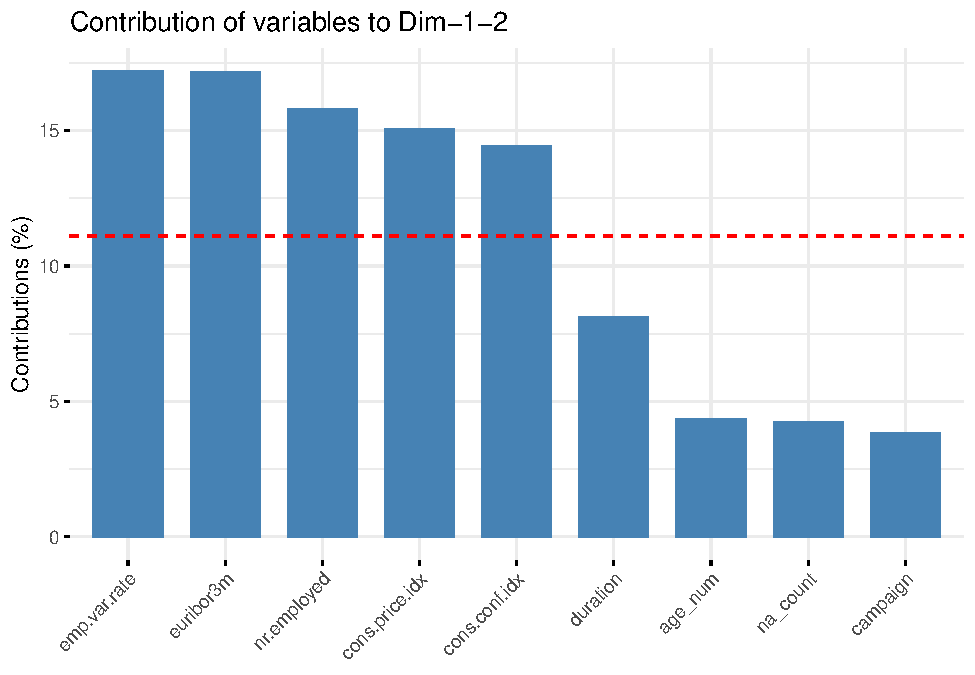
\includegraphics{Entrega2_files/figure-latex/unnamed-chunk-4-1.pdf}

\begin{Shaded}
\begin{Highlighting}[]
\NormalTok{mm }\OtherTok{\textless{}{-}} \FunctionTok{mean}\NormalTok{(res.ca1}\SpecialCharTok{$}\NormalTok{eig[,}\DecValTok{1}\NormalTok{])}
\NormalTok{ll}\OtherTok{\textless{}{-}} \FunctionTok{which}\NormalTok{(}\FunctionTok{as.data.frame}\NormalTok{(res.ca1}\SpecialCharTok{$}\NormalTok{eig[,}\DecValTok{1}\NormalTok{])}\SpecialCharTok{\textgreater{}}\NormalTok{mm)}
\FunctionTok{length}\NormalTok{(ll) }\CommentTok{\#Número dimensions}
\end{Highlighting}
\end{Shaded}

\begin{verbatim}
## [1] 2
\end{verbatim}

\begin{Shaded}
\begin{Highlighting}[]
\NormalTok{res.ca1}\SpecialCharTok{$}\NormalTok{eig[}\FunctionTok{length}\NormalTok{(ll),}\DecValTok{3}\NormalTok{]}
\end{Highlighting}
\end{Shaded}

\begin{verbatim}
## [1] 78.27887
\end{verbatim}

Gràficament, per la regla del colze, veiem que la dimensió on hi ha un
canvi important de la corva és la 2. A més, per Kaiser, agafem totes les
dimensions amb els eigenvalues els quals superin la mitjana de tots els
eigenvalues, i també ens surten dues dimensions.

Amb dues dimensions representem un 78.2788744\%, un percentatge prou
considerable.

\begin{Shaded}
\begin{Highlighting}[]
\FunctionTok{plot}\NormalTok{( res.ca1, }\AttributeTok{cex=}\FloatTok{0.8}\NormalTok{, }\AttributeTok{graph.type =} \StringTok{"classic"}\NormalTok{ )}
\FunctionTok{lines}\NormalTok{( res.ca1}\SpecialCharTok{$}\NormalTok{row}\SpecialCharTok{$}\NormalTok{coord[,}\DecValTok{1}\NormalTok{], res.ca1}\SpecialCharTok{$}\NormalTok{row}\SpecialCharTok{$}\NormalTok{coord[,}\DecValTok{2}\NormalTok{], }\AttributeTok{col=}\StringTok{"blue"}\NormalTok{, }\AttributeTok{lwd =} \DecValTok{2}\NormalTok{ )}
\FunctionTok{lines}\NormalTok{( res.ca1}\SpecialCharTok{$}\NormalTok{col}\SpecialCharTok{$}\NormalTok{coord[,}\DecValTok{1}\NormalTok{], res.ca1}\SpecialCharTok{$}\NormalTok{col}\SpecialCharTok{$}\NormalTok{coord[,}\DecValTok{2}\NormalTok{], }\AttributeTok{col=}\StringTok{"red"}\NormalTok{, }\AttributeTok{lwd =} \DecValTok{2}\NormalTok{ )}
\end{Highlighting}
\end{Shaded}

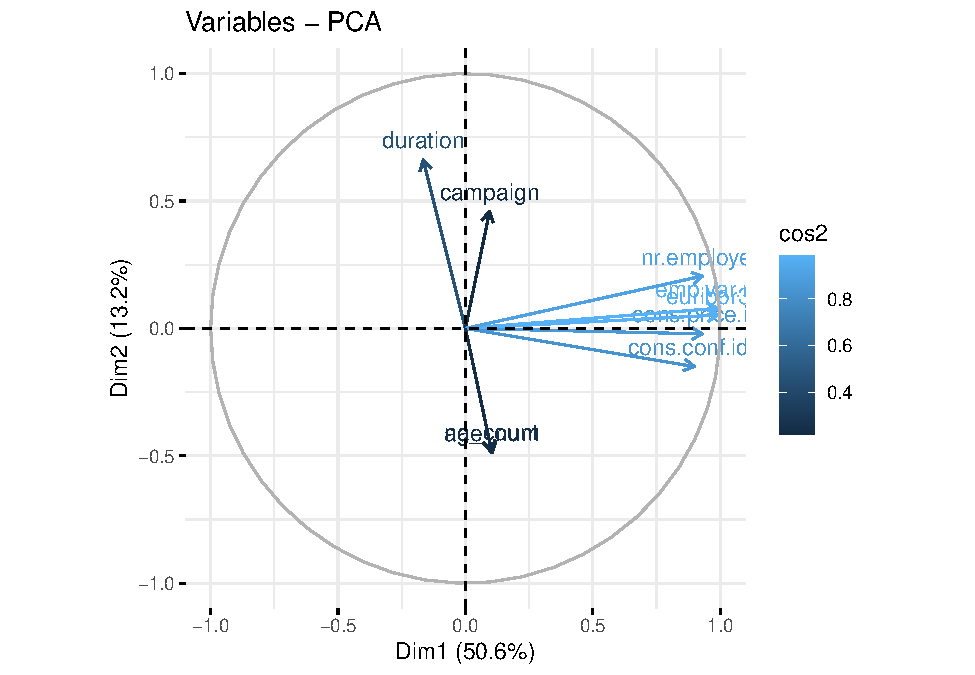
\includegraphics{Entrega2_files/figure-latex/unnamed-chunk-5-1.pdf}

Tal i com podem veure a la gràfica, hi ha diverses categories amb valors
molt similars, que, per tant, podriem considerar-les com a una sola. Per
exemple la duration\_fact curta i molt.curta tenen quasibé el mateix
valor, la resta de categories tenen prou discrepància. Mencionar que en
la variable job, tenim dues altres categories amb valors molt similars,
que són services i self-employed.

Podem observar que les feines amb posicions superiors tendeixen a estar
més estona a la trucada, mentres que els unemployed estan totalment
separats.

\hypertarget{duration_fact---education}{%
\paragraph{Duration\_fact - Education}\label{duration_fact---education}}

Igual que amb la parella anterior, realitzem la taula que relaciona les
dues variables i fem l'anàlisis de correspondència (CA).

\begin{Shaded}
\begin{Highlighting}[]
\NormalTok{df}\SpecialCharTok{$}\NormalTok{education }\OtherTok{\textless{}{-}} \FunctionTok{factor}\NormalTok{(df}\SpecialCharTok{$}\NormalTok{education, }\AttributeTok{levels =} \FunctionTok{c}\NormalTok{( }\StringTok{"illiterate"}\NormalTok{, }\StringTok{"basic"}\NormalTok{,}
                                                 \StringTok{"high.school"}\NormalTok{, }
                                                 \StringTok{"professional.course"}\NormalTok{, }
                                                 \StringTok{"university.degree"}\NormalTok{))}
\NormalTok{tab2 }\OtherTok{\textless{}{-}} \FunctionTok{table}\NormalTok{(df[,}\FunctionTok{c}\NormalTok{(}\StringTok{"duration\_fact"}\NormalTok{, }\StringTok{"education"}\NormalTok{)])}
\NormalTok{tab2}
\end{Highlighting}
\end{Shaded}

\begin{verbatim}
##              education
## duration_fact illiterate basic high.school professional.course
##   extr.curt            0     4           1                   1
##   molt.curta           0    26          16                   5
##   curta                0    57          26                  15
##   normal               0   769         529                 283
##   llarga               2   669         475                 250
##   molt.llarga          0   230         159                  73
##   extr.llarga          0    12           6                   5
##              education
## duration_fact university.degree
##   extr.curt                   2
##   molt.curta                 12
##   curta                      26
##   normal                    547
##   llarga                    605
##   molt.llarga               190
##   extr.llarga                 5
\end{verbatim}

\begin{Shaded}
\begin{Highlighting}[]
\NormalTok{res.ca2 }\OtherTok{\textless{}{-}} \FunctionTok{CA}\NormalTok{(tab2, }\AttributeTok{graph =}\NormalTok{ F)}
\end{Highlighting}
\end{Shaded}

Seguidament triarem les dimensions que hem d'agafar, gràficament i a
partir dels eigenvalues.

\begin{Shaded}
\begin{Highlighting}[]
\FunctionTok{fviz\_eig}\NormalTok{(res.ca2)}
\end{Highlighting}
\end{Shaded}

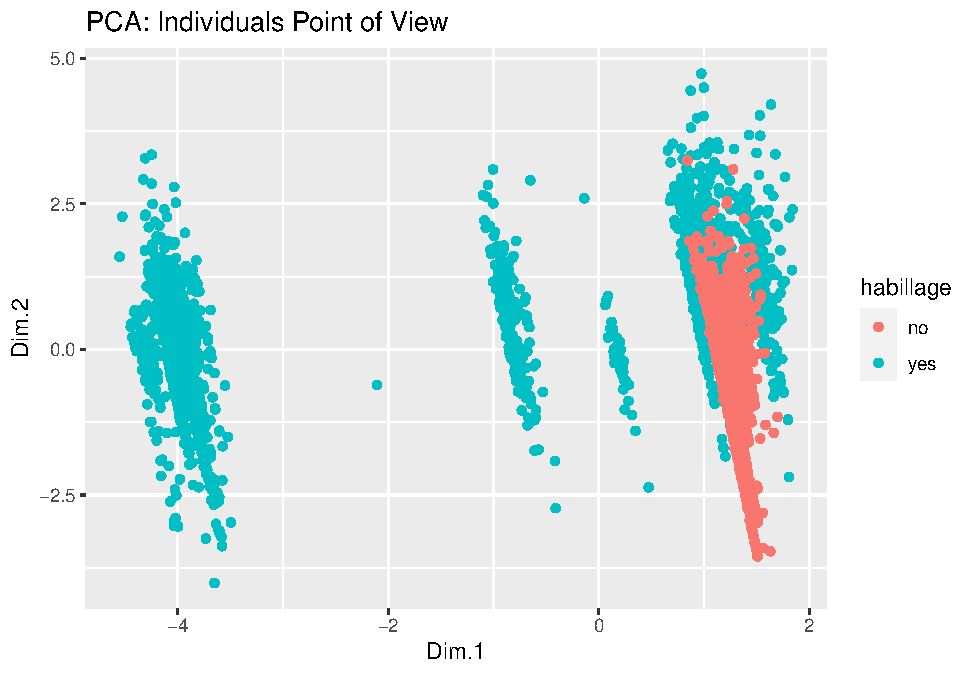
\includegraphics{Entrega2_files/figure-latex/unnamed-chunk-7-1.pdf}

\begin{Shaded}
\begin{Highlighting}[]
\NormalTok{mm }\OtherTok{\textless{}{-}} \FunctionTok{mean}\NormalTok{(res.ca2}\SpecialCharTok{$}\NormalTok{eig[,}\DecValTok{1}\NormalTok{])}
\NormalTok{ll}\OtherTok{\textless{}{-}} \FunctionTok{which}\NormalTok{(}\FunctionTok{as.data.frame}\NormalTok{(res.ca2}\SpecialCharTok{$}\NormalTok{eig[,}\DecValTok{1}\NormalTok{])}\SpecialCharTok{\textgreater{}}\NormalTok{mm)}
\FunctionTok{length}\NormalTok{(ll) }\CommentTok{\#Número dimensions}
\end{Highlighting}
\end{Shaded}

\begin{verbatim}
## [1] 1
\end{verbatim}

\begin{Shaded}
\begin{Highlighting}[]
\NormalTok{res.ca2}\SpecialCharTok{$}\NormalTok{eig[}\FunctionTok{length}\NormalTok{(ll),}\DecValTok{3}\NormalTok{]}
\end{Highlighting}
\end{Shaded}

\begin{verbatim}
## [1] 74.3226
\end{verbatim}

Gràficament, per la regla del colze, veiem que la dimensió on hi ha un
canvi important de la corva és la 1. A més, per Kaiser, agafem totes les
dimensions amb els eigenvalues els quals superin la mitjana de tots els
eigenvalues, i també ens surt una sola dimensió.

Amb aquesta dimensions representem un 74.3226032\%, de nou un
percentatge prou considerable.

\begin{Shaded}
\begin{Highlighting}[]
\FunctionTok{plot}\NormalTok{( res.ca2, }\AttributeTok{cex=}\FloatTok{0.8}\NormalTok{, }\AttributeTok{graph.type =} \StringTok{"classic"}\NormalTok{ )}
\FunctionTok{lines}\NormalTok{( res.ca2}\SpecialCharTok{$}\NormalTok{row}\SpecialCharTok{$}\NormalTok{coord[,}\DecValTok{1}\NormalTok{], res.ca2}\SpecialCharTok{$}\NormalTok{row}\SpecialCharTok{$}\NormalTok{coord[,}\DecValTok{2}\NormalTok{], }\AttributeTok{col=}\StringTok{"blue"}\NormalTok{, }\AttributeTok{lwd =} \DecValTok{2}\NormalTok{ )}
\FunctionTok{lines}\NormalTok{( res.ca2}\SpecialCharTok{$}\NormalTok{col}\SpecialCharTok{$}\NormalTok{coord[,}\DecValTok{1}\NormalTok{], res.ca2}\SpecialCharTok{$}\NormalTok{col}\SpecialCharTok{$}\NormalTok{coord[,}\DecValTok{2}\NormalTok{], }\AttributeTok{col=}\StringTok{"red"}\NormalTok{, }\AttributeTok{lwd =} \DecValTok{2}\NormalTok{ )}
\end{Highlighting}
\end{Shaded}

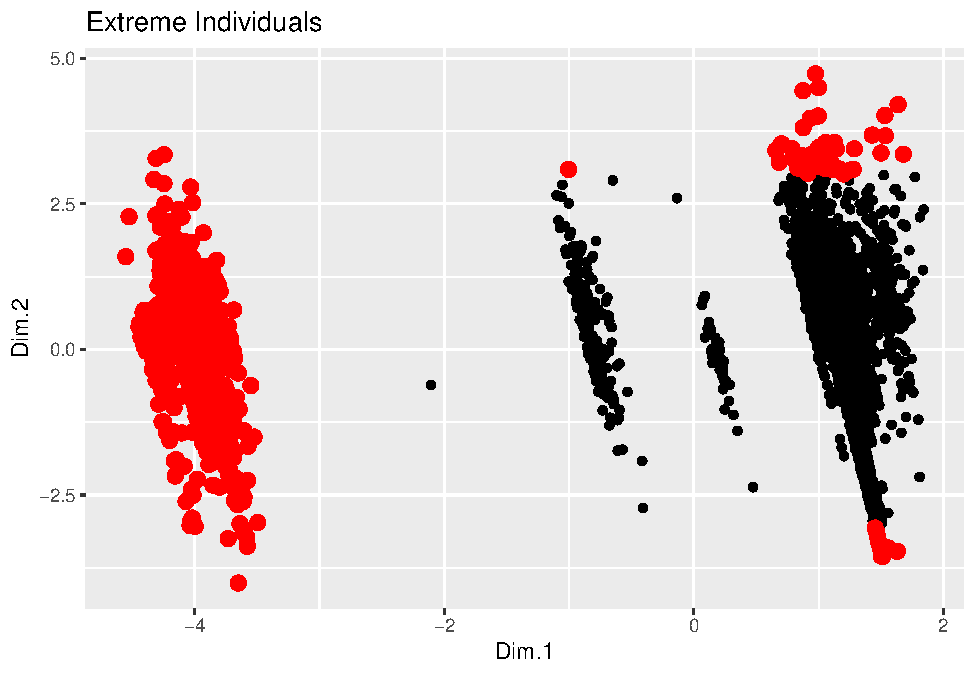
\includegraphics{Entrega2_files/figure-latex/unnamed-chunk-8-1.pdf}

De la mateixa forma que hem vist amb la parella de variables anterior,
aquí tornem a veure que les categories de duration\_fact curta i
molt.curta tenen valors molt similars. A més, veiem que llarga i
molt.llarga també els passa el mateix.

Ens podem fixar també amb que la categoria de education illiterate està
molt separada de la resta, cosa que té molt de sentit. De la mateixa
manera podem veure que els nivells d'estudi més alts estan relacionats
amb les trucades més llargues.

\hypertarget{anuxe0lisis-mca}{%
\subsection{Anàlisis MCA}\label{anuxe0lisis-mca}}

\begin{Shaded}
\begin{Highlighting}[]
\NormalTok{llmout}\OtherTok{\textless{}{-}}\FunctionTok{which}\NormalTok{(df}\SpecialCharTok{$}\NormalTok{mout}\SpecialCharTok{==}\StringTok{"Yes"}\NormalTok{)}
\NormalTok{res.mca}\OtherTok{\textless{}{-}}\FunctionTok{MCA}\NormalTok{(df[,}\FunctionTok{c}\NormalTok{(var\_res, var\_dis[}\DecValTok{1}\SpecialCharTok{:}\DecValTok{11}\NormalTok{]) ], }\AttributeTok{quali.sup=}\DecValTok{1}\NormalTok{, }\AttributeTok{ind.sup=}\NormalTok{llmout,}
             \AttributeTok{graph =}\NormalTok{ F)}
\end{Highlighting}
\end{Shaded}

\hypertarget{eigenvalues-and-dominant-axes.-how-many-axes-we-have-to-consider-for-next-hierarchical-classification-stage}{%
\subsubsection{1. Eigenvalues and dominant axes. How many axes we have
to consider for next Hierarchical Classification
stage?}\label{eigenvalues-and-dominant-axes.-how-many-axes-we-have-to-consider-for-next-hierarchical-classification-stage}}

En aquest primer punt haurem d'escollir les dimensions que agafem per
fer l'anàlisis a partir dels eigenvalues. Per a triar les dimensions
durem a terme dos mètodes, el de Kaiser i el de la regla del colze:

\hypertarget{regla-de-kaiser}{%
\paragraph{Regla de Kaiser}\label{regla-de-kaiser}}

La regla de Kaiser ens diu que haurem d'agafar totes aquelles dimensions
amb el valor del eigenvalue superior al de la mitjana d'eigenvalues de
totes les dimensions.

\begin{Shaded}
\begin{Highlighting}[]
\FunctionTok{summary}\NormalTok{(res.mca, }\AttributeTok{nbelements =} \DecValTok{12}\NormalTok{, }\AttributeTok{nbind =} \DecValTok{0}\NormalTok{)}
\end{Highlighting}
\end{Shaded}

\begin{verbatim}
## 
## Call:
## MCA(X = df[, c(var_res, var_dis[1:11])], ind.sup = llmout, quali.sup = 1,  
##      graph = F) 
## 
## 
## Eigenvalues
##                        Dim.1   Dim.2   Dim.3   Dim.4   Dim.5   Dim.6   Dim.7
## Variance               0.216   0.175   0.147   0.142   0.135   0.122   0.115
## % of var.              7.200   5.838   4.900   4.740   4.493   4.076   3.848
## Cumulative % of var.   7.200  13.037  17.938  22.678  27.171  31.248  35.095
##                        Dim.8   Dim.9  Dim.10  Dim.11  Dim.12  Dim.13  Dim.14
## Variance               0.107   0.102   0.099   0.098   0.096   0.095   0.094
## % of var.              3.574   3.416   3.316   3.279   3.197   3.151   3.117
## Cumulative % of var.  38.669  42.085  45.401  48.680  51.877  55.028  58.145
##                       Dim.15  Dim.16  Dim.17  Dim.18  Dim.19  Dim.20  Dim.21
## Variance               0.092   0.091   0.090   0.088   0.087   0.084   0.082
## % of var.              3.077   3.034   2.989   2.934   2.884   2.815   2.724
## Cumulative % of var.  61.222  64.257  67.246  70.180  73.064  75.879  78.603
##                       Dim.22  Dim.23  Dim.24  Dim.25  Dim.26  Dim.27  Dim.28
## Variance               0.081   0.080   0.077   0.076   0.068   0.060   0.055
## % of var.              2.688   2.677   2.582   2.538   2.266   2.001   1.831
## Cumulative % of var.  81.291  83.968  86.550  89.088  91.354  93.355  95.186
##                       Dim.29  Dim.30  Dim.31  Dim.32  Dim.33
## Variance               0.050   0.043   0.030   0.019   0.002
## % of var.              1.661   1.428   1.009   0.647   0.070
## Cumulative % of var.  96.846  98.274  99.283  99.930 100.000
## 
## Categories (the 12 first)
##                   Dim.1     ctr    cos2  v.test     Dim.2     ctr    cos2
## Jove          |   0.877   1.101   0.027  11.565 |  -0.711   0.892   0.018
## Jove-Adult    |   0.038   0.042   0.003   3.964 |  -0.058   0.119   0.007
## Adult         |  -0.239   0.662   0.022 -10.349 |   0.244   0.851   0.023
## Gran          |   1.597   0.652   0.016   8.772 |  -0.551   0.096   0.002
## admin.        |   0.438   1.896   0.059  17.051 |  -0.458   2.554   0.064
## blue-collar   |  -0.667   4.847   0.155 -27.700 |   0.674   6.101   0.159
## management    |   0.132   0.056   0.001   2.664 |  -0.397   0.621   0.013
## self-employed |   0.111   0.036   0.001   2.140 |  -0.222   0.180   0.004
## services      |  -0.192   0.165   0.004  -4.650 |   0.020   0.002   0.000
## technician    |   0.362   0.838   0.023  10.764 |  -0.129   0.131   0.003
## unemployed    |   0.170   0.125   0.003   4.036 |  -0.036   0.007   0.000
## divorced      |   0.010   0.000   0.000   0.235 |  -0.179   0.175   0.004
##                v.test     Dim.3     ctr    cos2  v.test  
## Jove           -9.373 |  -0.520   0.569   0.010  -6.859 |
## Jove-Adult     -5.989 |  -0.220   2.056   0.106 -22.849 |
## Adult          10.565 |   0.517   4.535   0.101  22.345 |
## Gran           -3.024 |   4.408   7.298   0.119  24.216 |
## admin.        -17.818 |  -0.540   4.236   0.090 -21.025 |
## blue-collar    27.984 |   0.623   6.208   0.135  25.862 |
## management     -7.998 |   0.121   0.068   0.001   2.430 |
## self-employed  -4.294 |   0.290   0.366   0.006   5.611 |
## services        0.480 |  -1.350  11.974   0.217 -32.712 |
## technician     -3.835 |  -0.098   0.089   0.002  -2.901 |
## unemployed     -0.861 |   0.919   5.360   0.097  21.841 |
## divorced       -4.321 |  -0.013   0.001   0.000  -0.318 |
## 
## Categorical variables (eta2)
##                 Dim.1 Dim.2 Dim.3  
## age           | 0.058 0.038 0.234 |
## job           | 0.189 0.185 0.458 |
## marital       | 0.104 0.084 0.090 |
## education     | 0.203 0.215 0.427 |
## housing       | 0.030 0.005 0.025 |
## loan          | 0.002 0.001 0.000 |
## contact       | 0.528 0.049 0.109 |
## month         | 0.488 0.135 0.152 |
## day_of_week   | 0.062 0.014 0.025 |
## previous      | 0.327 0.594 0.030 |
## poutcome      | 0.384 0.606 0.067 |
## 
## Supplementary categories
##                   Dim.1    cos2  v.test     Dim.2    cos2  v.test     Dim.3
## y_no          |  -0.585   0.375 -43.036 |   0.192   0.040  14.131 |  -0.241
## y_yes         |   0.641   0.375  43.036 |  -0.210   0.040 -14.131 |   0.264
##                  cos2  v.test  
## y_no            0.064 -17.713 |
## y_yes           0.064  17.713 |
## 
## Supplementary categorical variables (eta2)
##                 Dim.1 Dim.2 Dim.3  
## y             | 0.375 0.040 0.064 |
\end{verbatim}

\begin{Shaded}
\begin{Highlighting}[]
\NormalTok{mm }\OtherTok{\textless{}{-}} \FunctionTok{mean}\NormalTok{(res.mca}\SpecialCharTok{$}\NormalTok{eig[,}\DecValTok{1}\NormalTok{])}
\NormalTok{ll}\OtherTok{\textless{}{-}} \FunctionTok{which}\NormalTok{(}\FunctionTok{as.data.frame}\NormalTok{(res.mca}\SpecialCharTok{$}\NormalTok{eig[,}\DecValTok{1}\NormalTok{])}\SpecialCharTok{\textgreater{}}\NormalTok{mm)}
\FunctionTok{length}\NormalTok{(ll) }\CommentTok{\#Número dimensions}
\end{Highlighting}
\end{Shaded}

\begin{verbatim}
## [1] 16
\end{verbatim}

\begin{Shaded}
\begin{Highlighting}[]
\NormalTok{res.mca}\SpecialCharTok{$}\NormalTok{eig[}\FunctionTok{length}\NormalTok{(ll),}\DecValTok{3}\NormalTok{]}
\end{Highlighting}
\end{Shaded}

\begin{verbatim}
## [1] 64.25661
\end{verbatim}

\begin{Shaded}
\begin{Highlighting}[]
\FunctionTok{barplot}\NormalTok{(res.mca}\SpecialCharTok{$}\NormalTok{eig[,}\DecValTok{1}\NormalTok{],}
        \AttributeTok{main=}\StringTok{"valors propis"}\NormalTok{,}
        \AttributeTok{names.arg=}\FunctionTok{paste}\NormalTok{(}\StringTok{"dim"}\NormalTok{,}\DecValTok{1}\SpecialCharTok{:}\FunctionTok{nrow}\NormalTok{(res.mca}\SpecialCharTok{$}\NormalTok{eig)),}
        \AttributeTok{las =} \DecValTok{2}\NormalTok{,}
        \AttributeTok{ylim =} \FunctionTok{c}\NormalTok{(}\DecValTok{0}\NormalTok{, }\FloatTok{0.25}\NormalTok{),}
        \AttributeTok{col =} \StringTok{"blue4"}\NormalTok{)}

\FunctionTok{abline}\NormalTok{(}\AttributeTok{h =}\NormalTok{ mm,}
       \AttributeTok{col =} \StringTok{"red"}\NormalTok{,}
       \AttributeTok{lty =} \StringTok{"dashed"}\NormalTok{)}
\end{Highlighting}
\end{Shaded}

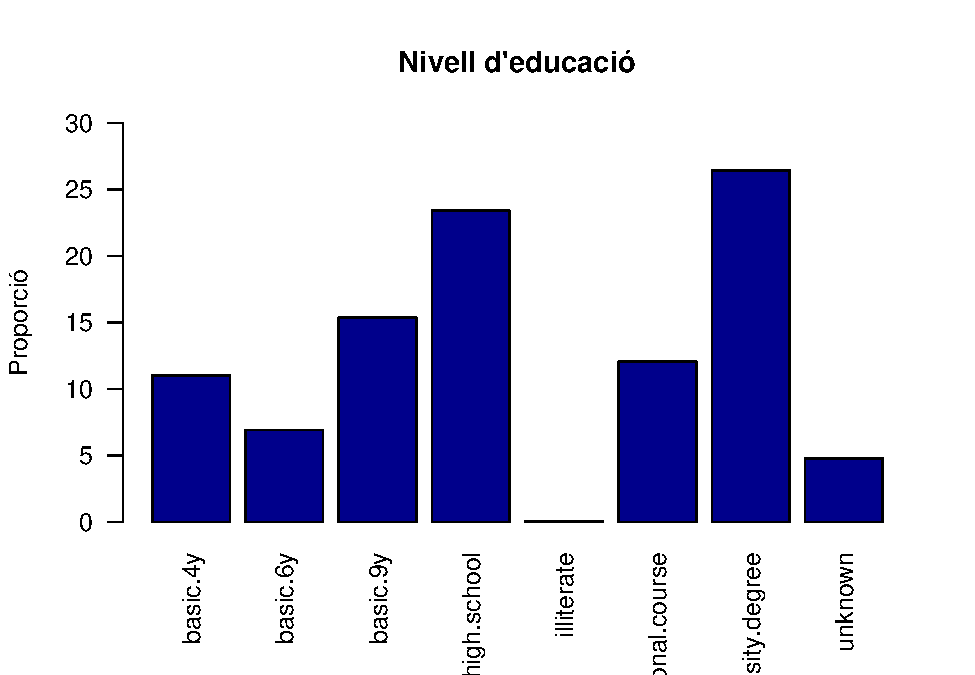
\includegraphics{Entrega2_files/figure-latex/unnamed-chunk-10-1.pdf}

Per la regla de Kaiser ens surten 16 dimensions, però el percentatge
explicat és 64.2566121\%, un percentatge que considerem baix.

\hypertarget{regla-del-colze}{%
\paragraph{Regla del colze}\label{regla-del-colze}}

La regla del colze ens diu que hem d'agafar la dimensió la qual fa
variar la corva de la gràfica que ens indica el valor propi de cada
dimensió:

\begin{Shaded}
\begin{Highlighting}[]
\NormalTok{res.mca}\SpecialCharTok{$}\NormalTok{eig}
\end{Highlighting}
\end{Shaded}

\begin{verbatim}
##         eigenvalue percentage of variance cumulative percentage of variance
## dim 1  0.215985532              7.1995177                          7.199518
## dim 2  0.175136654              5.8378885                         13.037406
## dim 3  0.147012791              4.9004264                         17.937833
## dim 4  0.142213865              4.7404622                         22.678295
## dim 5  0.134796116              4.4932039                         27.171499
## dim 6  0.122285019              4.0761673                         31.247666
## dim 7  0.115427448              3.8475816                         35.095247
## dim 8  0.107226255              3.5742085                         38.669456
## dim 9  0.102473603              3.4157868                         42.085243
## dim 10 0.099474533              3.3158178                         45.401061
## dim 11 0.098357758              3.2785919                         48.679652
## dim 12 0.095920509              3.1973503                         51.877003
## dim 13 0.094527756              3.1509252                         55.027928
## dim 14 0.093515471              3.1171824                         58.145110
## dim 15 0.092316196              3.0772065                         61.222317
## dim 16 0.091028857              3.0342952                         64.256612
## dim 17 0.089676076              2.9892025                         67.245815
## dim 18 0.088030654              2.9343551                         70.180170
## dim 19 0.086521870              2.8840623                         73.064232
## dim 20 0.084453327              2.8151109                         75.879343
## dim 21 0.081712085              2.7237362                         78.603079
## dim 22 0.080640389              2.6880130                         81.291092
## dim 23 0.080312899              2.6770966                         83.968189
## dim 24 0.077456392              2.5818797                         86.550068
## dim 25 0.076140285              2.5380095                         89.088078
## dim 26 0.067968101              2.2656034                         91.353681
## dim 27 0.060034342              2.0011447                         93.354826
## dim 28 0.054925787              1.8308596                         95.185686
## dim 29 0.049820820              1.6606940                         96.846380
## dim 30 0.042831485              1.4277162                         98.274096
## dim 31 0.030266658              1.0088886                         99.282984
## dim 32 0.019421634              0.6473878                         99.930372
## dim 33 0.002088834              0.0696278                        100.000000
\end{verbatim}

\begin{Shaded}
\begin{Highlighting}[]
\FunctionTok{fviz\_screeplot}\NormalTok{(res.mca,}
               \AttributeTok{ylim =} \FunctionTok{c}\NormalTok{(}\DecValTok{0}\NormalTok{, }\DecValTok{8}\NormalTok{),}
               \AttributeTok{ncp =} \DecValTok{33}\NormalTok{)}
\end{Highlighting}
\end{Shaded}

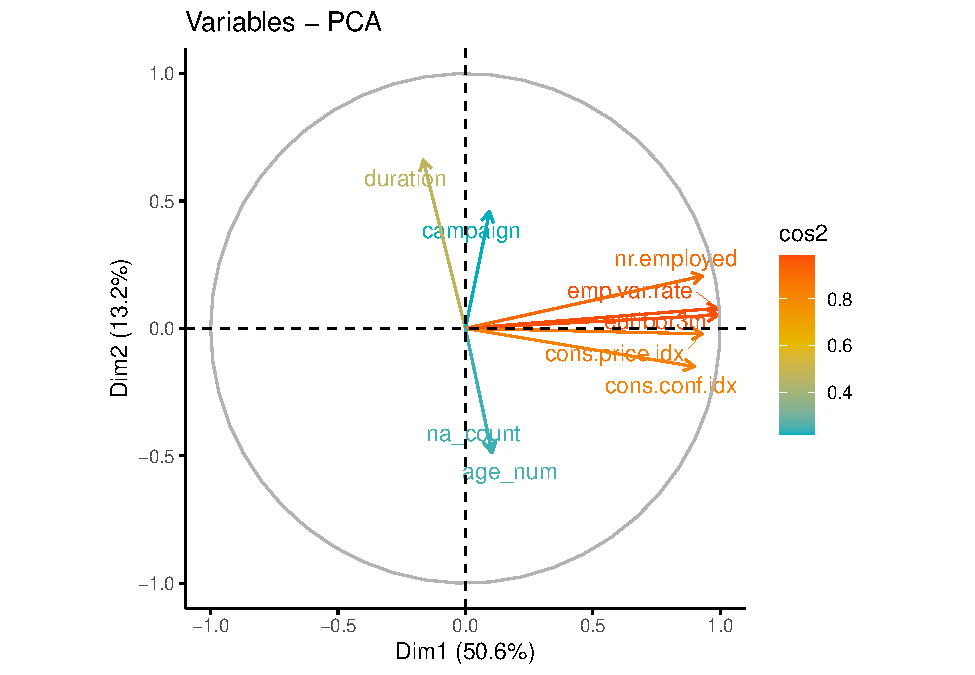
\includegraphics{Entrega2_files/figure-latex/unnamed-chunk-11-1.pdf}

En el nostre cas, agafarem la primera dimensió que té un percentatge
acomulat de variança més gran de 85\%, la dimensió 24. Podem veure
gràficament com aquesta dimensió és la última que manté una corva de
valor propi constant i que ens explica suficient variança, a partir de
la dimensió 25 la corva canvia la seva linealitat.

\hypertarget{individuals-point-of-view}{%
\subsubsection{2. Individuals point of
view}\label{individuals-point-of-view}}

\begin{Shaded}
\begin{Highlighting}[]
\FunctionTok{plot}\NormalTok{(res.mca, }\AttributeTok{choix =} \FunctionTok{c}\NormalTok{(}\StringTok{"ind"}\NormalTok{),}
     \AttributeTok{invisible =} \FunctionTok{c}\NormalTok{(}\StringTok{"var"}\NormalTok{, }\StringTok{"quali.sup"}\NormalTok{),}
     \AttributeTok{cex =} \DecValTok{1}\NormalTok{)}
\end{Highlighting}
\end{Shaded}

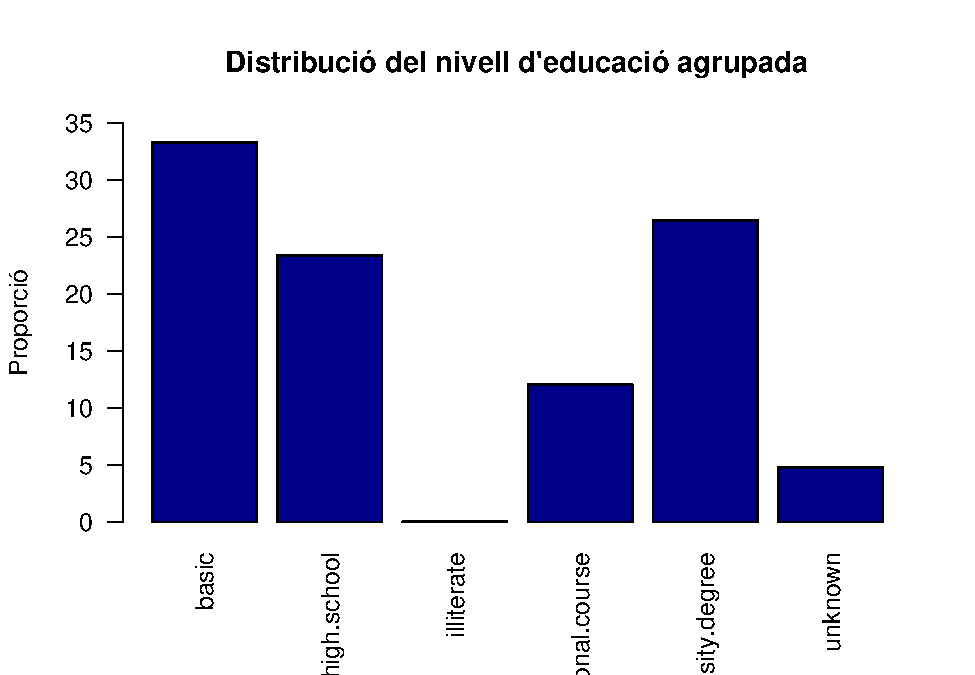
\includegraphics{Entrega2_files/figure-latex/unnamed-chunk-12-1.pdf}

Podem distingir dos grups diferenciats d'individus, un a l'origen de
coordenades i l'altre al primer quadrant, i un grup molt petit
d'individus entre ells. Tal i com veiem a la gràfica, el grup del primer
quadrant té una contribució molt superior als altres tan en la dimensió
1 com en la 2.

A continuació veurem els 10 individus que més contribueixen a explicar
la primera dimensió i quins valors tenen en les diferents variables:

\begin{Shaded}
\begin{Highlighting}[]
\NormalTok{inds }\OtherTok{\textless{}{-}}\NormalTok{ res.mca}\SpecialCharTok{$}\NormalTok{ind}\SpecialCharTok{$}\NormalTok{coord}
\NormalTok{inds }\OtherTok{\textless{}{-}} \FunctionTok{as.data.frame}\NormalTok{(inds)}
\NormalTok{rang}\OtherTok{\textless{}{-}}\NormalTok{inds[}\FunctionTok{order}\NormalTok{(inds}\SpecialCharTok{$}\StringTok{\textasciigrave{}}\AttributeTok{Dim 1}\StringTok{\textasciigrave{}}\NormalTok{, }\AttributeTok{decreasing =} \ConstantTok{TRUE}\NormalTok{),]}
\NormalTok{res.mca}\SpecialCharTok{$}\NormalTok{ind}\SpecialCharTok{$}\NormalTok{coord[}\FunctionTok{row.names}\NormalTok{(rang)[}\DecValTok{1}\SpecialCharTok{:}\DecValTok{10}\NormalTok{],}\DecValTok{1}\NormalTok{]}
\end{Highlighting}
\end{Shaded}

\begin{verbatim}
##    30418    30140    30419    30208    30189    29511    30150    30315 
## 2.609911 2.595063 2.570233 2.533980 2.522024 2.506387 2.488380 2.463199 
##    30185    30244 
## 2.454798 2.411644
\end{verbatim}

\begin{Shaded}
\begin{Highlighting}[]
\NormalTok{df[}\FunctionTok{which}\NormalTok{(}\FunctionTok{row.names}\NormalTok{(df) }\SpecialCharTok{\%in\%} \FunctionTok{row.names}\NormalTok{(res.mca}\SpecialCharTok{$}\NormalTok{ind}\SpecialCharTok{$}\NormalTok{coord}
\NormalTok{                                      [}\FunctionTok{row.names}\NormalTok{(rang)[}\DecValTok{1}\SpecialCharTok{:}\DecValTok{10}\NormalTok{],])),}\DecValTok{1}\SpecialCharTok{:}\DecValTok{20}\NormalTok{]}
\end{Highlighting}
\end{Shaded}

\begin{verbatim}
##              age           job marital           education housing loan
## 30189 Jove-Adult        admin.  single         high.school     yes   no
## 30315 Jove-Adult        admin. married   university.degree     yes   no
## 30208 Jove-Adult    technician  single professional.course     yes   no
## 30244 Jove-Adult    technician married professional.course     yes  yes
## 30419 Jove-Adult self-employed  single   university.degree     yes  yes
## 30150      Adult        admin.  single   university.degree      no   no
## 30140 Jove-Adult    technician  single   university.degree     yes   no
## 30185 Jove-Adult        admin.  single         high.school      no   no
## 30418 Jove-Adult        admin.  single   university.degree     yes   no
## 29511 Jove-Adult        admin.  single   university.degree     yes   no
##        contact month day_of_week duration campaign previous poutcome
## 30189 cellular   apr         thu      354        1      Yes  success
## 30315 cellular   apr         thu      483        1      Yes  success
## 30208 cellular   apr         thu      218        1      Yes  success
## 30244 cellular   apr         thu      266        2      Yes  success
## 30419 cellular   apr         thu      509        1      Yes  success
## 30150 cellular   apr         thu      494        1      Yes  success
## 30140 cellular   apr         thu      701        1      Yes  success
## 30185 cellular   apr         thu      252        1      Yes  success
## 30418 cellular   apr         thu      502        1      Yes  success
## 29511 cellular   apr         mon      670        4      Yes  success
##       emp.var.rate cons.price.idx cons.conf.idx euribor3m nr.employed   y
## 30189         -1.8         93.075         -47.1     1.365      5099.1 yes
## 30315         -1.8         93.075         -47.1     1.365      5099.1 yes
## 30208         -1.8         93.075         -47.1     1.365      5099.1 yes
## 30244         -1.8         93.075         -47.1     1.365      5099.1 yes
## 30419         -1.8         93.075         -47.1     1.365      5099.1 yes
## 30150         -1.8         93.075         -47.1     1.365      5099.1 yes
## 30140         -1.8         93.075         -47.1     1.365      5099.1 yes
## 30185         -1.8         93.075         -47.1     1.365      5099.1 yes
## 30418         -1.8         93.075         -47.1     1.365      5099.1 yes
## 29511         -1.8         93.075         -47.1     1.405      5099.1 yes
##       age_num
## 30189      45
## 30315      36
## 30208      36
## 30244      36
## 30419      40
## 30150      53
## 30140      31
## 30185      31
## 30418      30
## 29511      43
\end{verbatim}

Seguidament veurem la mateixa informació però per la segona dimensió:

\begin{Shaded}
\begin{Highlighting}[]
\NormalTok{rang}\OtherTok{\textless{}{-}}\NormalTok{inds[}\FunctionTok{order}\NormalTok{(inds}\SpecialCharTok{$}\StringTok{\textasciigrave{}}\AttributeTok{Dim 2}\StringTok{\textasciigrave{}}\NormalTok{, }\AttributeTok{decreasing =} \ConstantTok{TRUE}\NormalTok{),]}
\NormalTok{res.mca}\SpecialCharTok{$}\NormalTok{ind}\SpecialCharTok{$}\NormalTok{coord[}\FunctionTok{row.names}\NormalTok{(rang)[}\DecValTok{1}\SpecialCharTok{:}\DecValTok{10}\NormalTok{],}\DecValTok{2}\NormalTok{]}
\end{Highlighting}
\end{Shaded}

\begin{verbatim}
##    30596    34731    32721    33383    30473    28168    34408    34276 
## 2.998819 2.937982 2.930081 2.909436 2.898307 2.882058 2.872351 2.854547 
##    35942    28677 
## 2.846646 2.821221
\end{verbatim}

\begin{Shaded}
\begin{Highlighting}[]
\NormalTok{df[}\FunctionTok{which}\NormalTok{(}\FunctionTok{row.names}\NormalTok{(df) }\SpecialCharTok{\%in\%} \FunctionTok{row.names}\NormalTok{(res.mca}\SpecialCharTok{$}\NormalTok{ind}\SpecialCharTok{$}\NormalTok{coord}
\NormalTok{                                      [}\FunctionTok{row.names}\NormalTok{(rang)[}\DecValTok{1}\SpecialCharTok{:}\DecValTok{10}\NormalTok{],])),}\DecValTok{1}\SpecialCharTok{:}\DecValTok{20}\NormalTok{]}
\end{Highlighting}
\end{Shaded}

\begin{verbatim}
##              age         job marital education housing loan   contact month
## 28168 Jove-Adult blue-collar married     basic     yes   no telephone   apr
## 28677 Jove-Adult blue-collar married     basic      no   no  cellular   apr
## 32721      Adult blue-collar married     basic      no   no  cellular   may
## 34731      Adult blue-collar married     basic      no   no  cellular   may
## 30596      Adult blue-collar married     basic     yes   no telephone   may
## 35942 Jove-Adult blue-collar married     basic      no  yes  cellular   may
## 30473      Adult blue-collar married     basic     yes   no  cellular   may
## 34408 Jove-Adult blue-collar married     basic      no   no  cellular   may
## 33383      Adult blue-collar married     basic      no   no  cellular   may
## 34276 Jove-Adult blue-collar married     basic      no  yes  cellular   may
##       day_of_week duration campaign previous poutcome emp.var.rate
## 28168         mon     1353        2      Yes  success         -1.8
## 28677         thu      583        1      Yes  success         -1.8
## 32721         mon      474        1      Yes  success         -1.8
## 34731         thu      532        2      Yes  success         -1.8
## 30596         mon      483        4      Yes  success         -1.8
## 35942         mon      487        1      Yes  success         -1.8
## 30473         mon      293        3      Yes  success         -1.8
## 34408         thu      680        1      Yes  success         -1.8
## 33383         tue      309        1      Yes  success         -1.8
## 34276         thu      722        2      Yes  success         -1.8
##       cons.price.idx cons.conf.idx euribor3m nr.employed   y age_num
## 28168         93.075         -47.1     1.466      5099.1 yes      34
## 28677         93.075         -47.1     1.410      5099.1 yes      32
## 32721         92.893         -46.2     1.299      5099.1 yes      50
## 34731         92.893         -46.2     1.266      5099.1 yes      54
## 30596         92.893         -46.2     1.354      5099.1 yes      50
## 35942         92.893         -46.2     1.264      5099.1 yes      43
## 30473         92.893         -46.2     1.354      5099.1 yes      50
## 34408         92.893         -46.2     1.266      5099.1 yes      31
## 33383         92.893         -46.2     1.291      5099.1 yes      48
## 34276         92.893         -46.2     1.266      5099.1 yes      43
\end{verbatim}

A la següent gràfica podrem veure sobre sobre el pla quins individus son
els més contributius (marcats en vermell) i els menys (en groc).

\begin{Shaded}
\begin{Highlighting}[]
\CommentTok{\# A l\textquotesingle{}hora de fer les gràfiques per individus i categories,}
\CommentTok{\# posarem com a invisible els individus suplementaris per no tenir{-}los en}
\CommentTok{\# compte (individus amb outliers multivariants)}

\FunctionTok{fviz\_mca\_ind}\NormalTok{(}
\NormalTok{  res.mca,}
  \AttributeTok{geom=}\FunctionTok{c}\NormalTok{(}\StringTok{"point"}\NormalTok{),}
  \AttributeTok{col.ind=}\StringTok{"contrib"}\NormalTok{,}
  \AttributeTok{invisible=}\FunctionTok{c}\NormalTok{(}\StringTok{"ind.sup"}\NormalTok{),}
  \AttributeTok{gradient.cols=}\FunctionTok{c}\NormalTok{(}\StringTok{"yellow2"}\NormalTok{, }\StringTok{"red"}\NormalTok{)}
\NormalTok{)}
\end{Highlighting}
\end{Shaded}

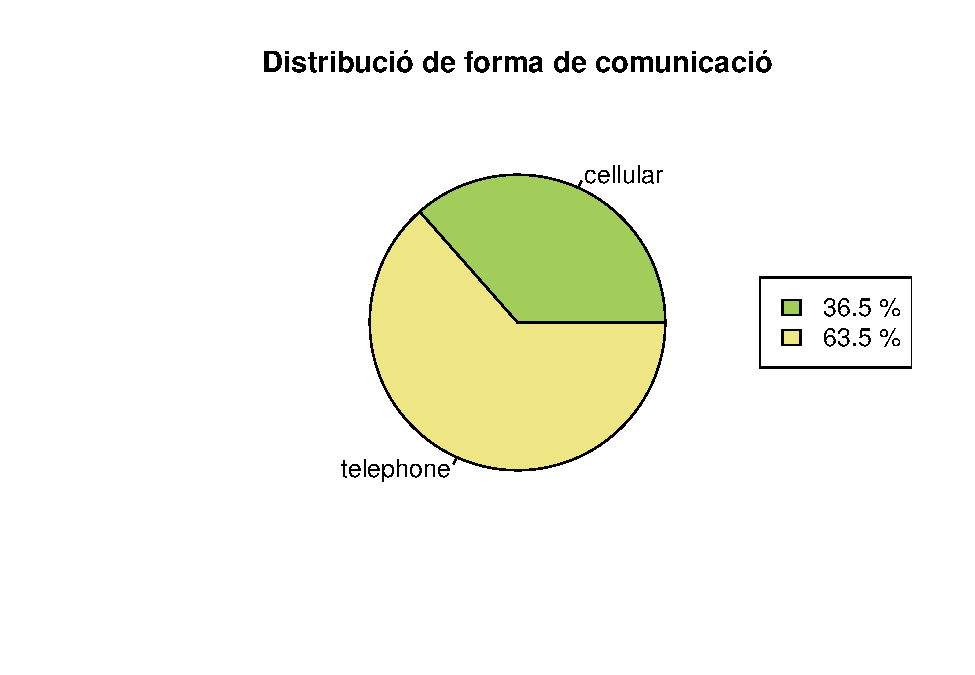
\includegraphics{Entrega2_files/figure-latex/unnamed-chunk-15-1.pdf}

\hypertarget{interpreting-map-of-categories}{%
\subsubsection{3. Interpreting map of
categories}\label{interpreting-map-of-categories}}

\begin{Shaded}
\begin{Highlighting}[]
\FunctionTok{fviz\_mca\_var}\NormalTok{(res.mca,}
             \AttributeTok{choice=}\StringTok{"mca.cor"}\NormalTok{,}
             \AttributeTok{repel =}\NormalTok{ T)}
\end{Highlighting}
\end{Shaded}

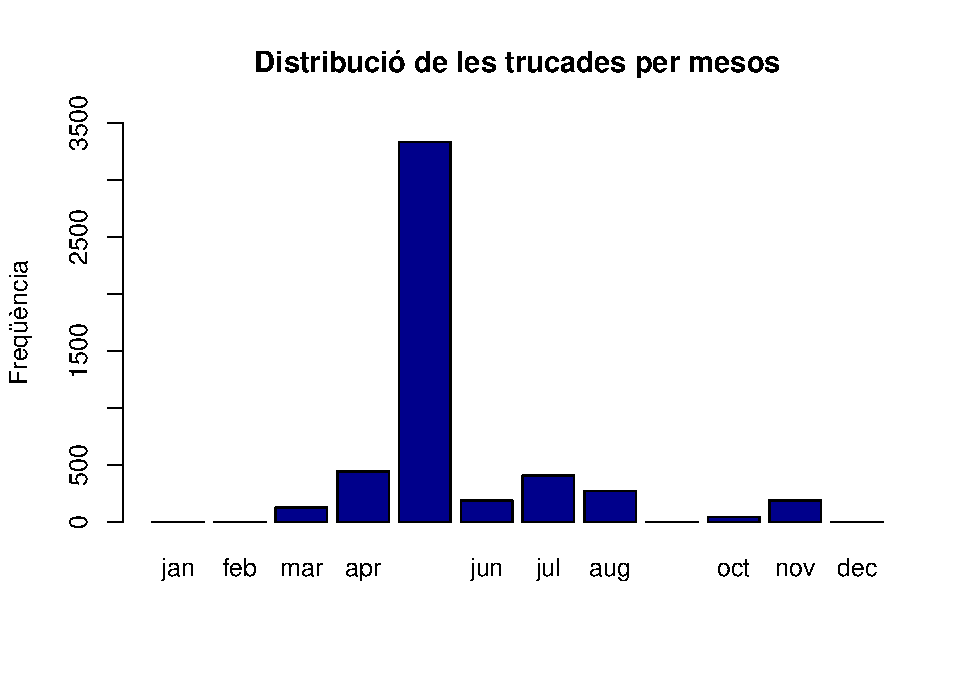
\includegraphics{Entrega2_files/figure-latex/unnamed-chunk-16-1.pdf}

Podem veure que contribueixen en gran mesura les variables previous i
poutcome per ambdues dimensions, mentres que per la dimensió 1 també
contribuieixen month i contact. Education i job tenen una contribució en
les dues dimensions en menor mesura de les mencionades anteriorment.

\begin{Shaded}
\begin{Highlighting}[]
\FunctionTok{fviz\_mca\_var}\NormalTok{(res.mca,}
             \AttributeTok{alpha.var=}\StringTok{"contrib"}\NormalTok{,}
             \AttributeTok{repel =}\NormalTok{ T)}
\end{Highlighting}
\end{Shaded}

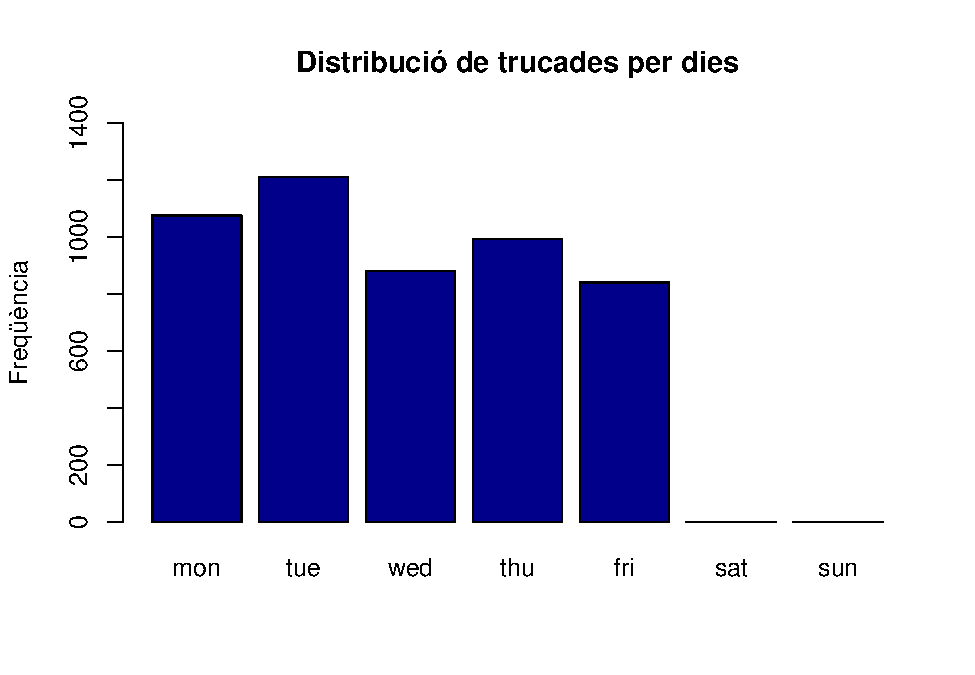
\includegraphics{Entrega2_files/figure-latex/unnamed-chunk-17-1.pdf}

Les categories més contributives en ambdues dimensions són ``success''
(categoria de ``poutcome'', variable que hem vist que contribuia en les
dues dimensions) i ``yes'' (categoria de previous que també contribuia
en les dues dimensions), la resta de categories no són tan determinants.

Representarem les categories de les variables més representatives:
poutcome, month i contact (com que poutcome i previous estan
relacionades, sols imprimirem la més significativa, és a dir, poutcome).

\begin{Shaded}
\begin{Highlighting}[]
\CommentTok{\# A l\textquotesingle{}hora de fer les gràfiques per individus i categories, posarem}
\CommentTok{\# com a invisible els individus suplementaris per no tenir{-}los en compte}
\CommentTok{\# (individus amb outliers multivariants)}
\FunctionTok{fviz\_mca\_ind}\NormalTok{(res.mca,}
             \AttributeTok{label=}\StringTok{"none"}\NormalTok{,}
             \AttributeTok{invisible=}\FunctionTok{c}\NormalTok{(}\StringTok{"ind.sup"}\NormalTok{),}
             \AttributeTok{geom =} \FunctionTok{c}\NormalTok{(}\StringTok{"point"}\NormalTok{),}
             \AttributeTok{habillage=}\StringTok{"poutcome"}\NormalTok{)}
\end{Highlighting}
\end{Shaded}

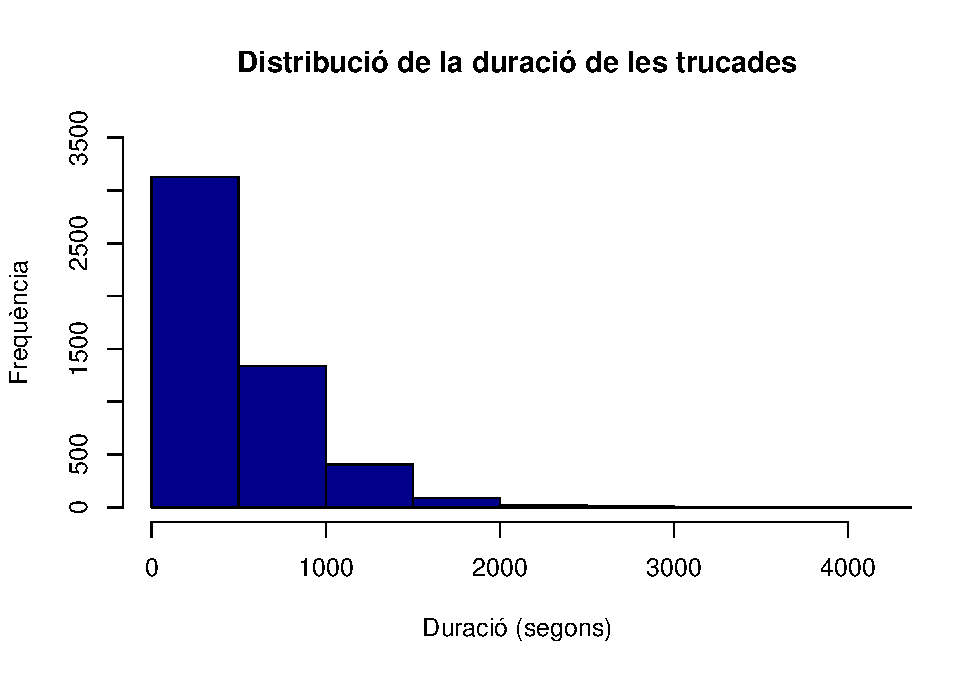
\includegraphics{Entrega2_files/figure-latex/unnamed-chunk-18-1.pdf}

\begin{Shaded}
\begin{Highlighting}[]
\FunctionTok{fviz\_mca\_ind}\NormalTok{(res.mca,}
             \AttributeTok{label=}\StringTok{"none"}\NormalTok{,}
             \AttributeTok{invisible=}\FunctionTok{c}\NormalTok{(}\StringTok{"ind.sup"}\NormalTok{),}
             \AttributeTok{geom =} \FunctionTok{c}\NormalTok{(}\StringTok{"point"}\NormalTok{),}
             \AttributeTok{habillage=}\StringTok{"contact"}\NormalTok{)}
\end{Highlighting}
\end{Shaded}

\includegraphics{Entrega2_files/figure-latex/unnamed-chunk-18-2.pdf}

\begin{Shaded}
\begin{Highlighting}[]
\FunctionTok{fviz\_mca\_ind}\NormalTok{(res.mca,}
             \AttributeTok{label=}\StringTok{"none"}\NormalTok{,}
             \AttributeTok{invisible=}\FunctionTok{c}\NormalTok{(}\StringTok{"ind.sup"}\NormalTok{),}
             \AttributeTok{geom =} \FunctionTok{c}\NormalTok{(}\StringTok{"point"}\NormalTok{),}
             \AttributeTok{habillage=}\StringTok{"month"}\NormalTok{)}
\end{Highlighting}
\end{Shaded}

\includegraphics{Entrega2_files/figure-latex/unnamed-chunk-18-3.pdf}

En els tres gràfics anteriors, podem veure com les categories formen
grups diferenciats, sobretot en les dues primeres. A la última gràfica
les categories no estan tan marcades, tot i que es veu una tendència
semblant entre categories.

\hypertarget{interpreting-the-axes-association-to-factor-map}{%
\subsubsection{4. Interpreting the axes association to factor
map}\label{interpreting-the-axes-association-to-factor-map}}

Per auquest punt durem a terme una descripció de dimensions a través de
la funció dimdesc per poder veure les variables i categories més
relacionades amb cada dimensió. Realitzarem l'anàlisis amb profunditat
de les tres primeres dimensions ja que són les més rellevants.

\begin{Shaded}
\begin{Highlighting}[]
\NormalTok{res.des }\OtherTok{\textless{}{-}} \FunctionTok{dimdesc}\NormalTok{(res.mca)}
\end{Highlighting}
\end{Shaded}

\hypertarget{dimensiuxf3-1}{%
\paragraph{Dimensió 1}\label{dimensiuxf3-1}}

\begin{Shaded}
\begin{Highlighting}[]
\NormalTok{res.des}\SpecialCharTok{$}\StringTok{\textasciigrave{}}\AttributeTok{Dim 1}\StringTok{\textasciigrave{}}\SpecialCharTok{$}\NormalTok{quali}
\end{Highlighting}
\end{Shaded}

\begin{verbatim}
##                      R2       p.value
## y           0.374987432  0.000000e+00
## contact     0.527902185  0.000000e+00
## month       0.488263590  0.000000e+00
## previous    0.327162493  0.000000e+00
## poutcome    0.384056740  0.000000e+00
## education   0.203105403 2.555766e-241
## job         0.189176924 2.541743e-220
## marital     0.104098708 1.426304e-118
## day_of_week 0.062267605  1.968206e-67
## age         0.058376451  4.596511e-64
## housing     0.029524225  4.813177e-34
## loan        0.001906531  2.143411e-03
\end{verbatim}

Les variables que més ens representan la primera dimensió són les
variables següents:

\begin{itemize}
\item
  contact (0.528)
\item
  month (0.488)
\item
  poutcome (0.384)
\end{itemize}

Aquestes tres variables són les que hem vist que estaven més
relacionades anteriorment de forma gràfica.

\begin{Shaded}
\begin{Highlighting}[]
\NormalTok{res.des}\SpecialCharTok{$}\StringTok{\textasciigrave{}}\AttributeTok{Dim 1}\StringTok{\textasciigrave{}}\SpecialCharTok{$}\NormalTok{category}
\end{Highlighting}
\end{Shaded}

\begin{verbatim}
##                                  Estimate       p.value
## poutcome=success               1.17531597  0.000000e+00
## previous=Yes                   1.01047661  0.000000e+00
## month=apr                      0.64675641  0.000000e+00
## contact=cellular               0.35132508  0.000000e+00
## y=y_yes                        0.28488898  0.000000e+00
## education=university.degree    0.05900022 2.383815e-128
## marital=single                 0.19670535 2.666734e-114
## job=admin.                     0.18013247  4.137677e-67
## day_of_week=thu                0.19339224  6.660628e-53
## month=mar                      0.46472456  6.802393e-45
## month=nov                      0.31200496  1.079628e-39
## month=aug                      0.22458575  4.665454e-37
## housing=housing_yes            0.07985867  4.813177e-34
## age=Jove                       0.14354196  2.506712e-31
## job=technician                 0.14485506  2.581261e-27
## month=jul                      0.10589318  1.029731e-24
## age=Gran                       0.47806017  1.307906e-18
## job=unemployed                 0.05540381  5.365573e-05
## loan=loan_yes                  0.02895621  2.143411e-03
## job=management                 0.03794035  7.710261e-03
## education=illiterate           0.63136693  1.235638e-02
## day_of_week=wed                0.02407510  2.879632e-02
## job=self-employed              0.02795219  3.237426e-02
## loan=loan_no                  -0.02895621  2.143411e-03
## education=high.school         -0.14980519  4.746968e-04
## day_of_week=mon               -0.05256369  3.291634e-04
## age=Jove-Adult                -0.24629074  7.288918e-05
## job=services                  -0.11268984  3.254931e-06
## education=professional.course -0.08612124  1.676784e-09
## month=jun                     -0.41903271  1.194469e-18
## age=Adult                     -0.37531139  2.372548e-25
## day_of_week=tue               -0.14817144  8.073767e-34
## housing=housing_no            -0.07985867  4.813177e-34
## poutcome=failure              -0.28388793  1.169020e-65
## marital=married               -0.15185866  6.566766e-96
## job=blue-collar               -0.33359402 2.665337e-183
## education=basic               -0.45444072 1.483351e-208
## poutcome=nonexistent          -0.89142804  0.000000e+00
## previous=No                   -1.01047661  0.000000e+00
## month=may                     -0.30916544  0.000000e+00
## contact=telephone             -0.35132508  0.000000e+00
## y=y_no                        -0.28488898  0.000000e+00
\end{verbatim}

Les categories que més representen la primera dimensió són les següents:

\begin{itemize}
\item
  success de poutcome (1.175)
\item
  Yes de previous (1.01)
\item
  apr de month (0.647)
\end{itemize}

Tot i que hi hagi contribucions negatives amb valors més destacats, no
els tenim en compte ja que són categories contràries a les que tenim en
positiu.

Aquestes tres categories són les que hem vist que estaven més
relacionades anteriorment de forma gràfica.

\hypertarget{dimensiuxf3-2}{%
\paragraph{Dimensió 2}\label{dimensiuxf3-2}}

\begin{Shaded}
\begin{Highlighting}[]
\NormalTok{res.des}\SpecialCharTok{$}\StringTok{\textasciigrave{}}\AttributeTok{Dim 2}\StringTok{\textasciigrave{}}\SpecialCharTok{$}\NormalTok{quali}
\end{Highlighting}
\end{Shaded}

\begin{verbatim}
##                       R2       p.value
## previous    0.5940564621  0.000000e+00
## poutcome    0.6062924147  0.000000e+00
## education   0.2149866672 2.160555e-257
## job         0.1848775504 1.122408e-214
## month       0.1351545003 2.072247e-149
## marital     0.0835207347  3.160431e-94
## contact     0.0494419477  2.166185e-56
## y           0.0404296938  3.143042e-46
## age         0.0377013815  7.044337e-41
## day_of_week 0.0142988220  1.337097e-14
## housing     0.0053479661  2.667713e-07
## loan        0.0008247522  4.355077e-02
\end{verbatim}

Les variables que més ens representan la segona dimensió són les
variables següents:

\begin{itemize}
\item
  poutcome (0.6062)
\item
  previous (0.5940)
\item
  education (0.215)
\end{itemize}

Aquestes tres variables són les que hem vist que estaven més
relacionades anteriorment de forma gràfica.

\begin{Shaded}
\begin{Highlighting}[]
\NormalTok{res.des}\SpecialCharTok{$}\StringTok{\textasciigrave{}}\AttributeTok{Dim 2}\StringTok{\textasciigrave{}}\SpecialCharTok{$}\NormalTok{category}
\end{Highlighting}
\end{Shaded}

\begin{verbatim}
##                                Estimate       p.value
## poutcome=success             1.73394719  0.000000e+00
## previous=Yes                 1.22612449  0.000000e+00
## education=basic              0.31810208 9.138533e-212
## job=blue-collar              0.31488937 2.189283e-187
## month=may                    0.17499654 1.506661e-102
## marital=married              0.14623996  1.751311e-89
## contact=telephone            0.09681807  2.166185e-56
## y=y_no                       0.08423522  3.143042e-46
## age=Adult                    0.21471233  2.315031e-26
## age=Jove-Adult               0.08827440  1.987533e-09
## education=high.school        0.01860896  9.527271e-09
## housing=housing_no           0.03060577  2.667713e-07
## day_of_week=thu              0.06294006  9.326999e-07
## day_of_week=mon              0.04771803  1.318104e-04
## loan=loan_no                 0.01714975  4.355077e-02
## loan=loan_yes               -0.01714975  4.355077e-02
## age=Gran                    -0.11796644  2.483794e-03
## month=oct                   -0.14489659  3.614771e-04
## job=technician              -0.02121630  1.242614e-04
## day_of_week=fri             -0.05220759  1.885359e-05
## job=self-employed           -0.06021933  1.728930e-05
## marital=divorced            -0.01775560  1.526968e-05
## housing=housing_yes         -0.03060577  2.667713e-07
## day_of_week=wed             -0.06639553  4.421294e-08
## poutcome=failure            -0.95300863  1.250230e-12
## job=management              -0.13337023  1.030364e-15
## age=Jove                    -0.18502029  4.814380e-21
## month=nov                   -0.22143499  4.994564e-25
## month=mar                   -0.32129786  3.766175e-27
## month=jul                   -0.13918909  2.462041e-29
## month=aug                   -0.25156750  4.941531e-43
## y=y_yes                     -0.08423522  3.143042e-46
## contact=cellular            -0.09681807  2.166185e-56
## job=admin.                  -0.15882870  2.586561e-73
## marital=single              -0.12848436  1.929238e-79
## poutcome=nonexistent        -0.78093856 6.075965e-139
## education=university.degree -0.16532509 8.613027e-153
## previous=No                 -1.22612449  0.000000e+00
\end{verbatim}

Les categories que més representen la segona dimensió són les següents:

\begin{itemize}
\item
  success de poutcome (1.734)
\item
  Yes de previous (1.226)
\item
  basic de education (0.318)
\end{itemize}

Aquestes tres categories són les que hem vist que estaven més
relacionades anteriorment de forma gràfica.

\hypertarget{dimensiuxf3-3}{%
\paragraph{Dimensió 3}\label{dimensiuxf3-3}}

\begin{Shaded}
\begin{Highlighting}[]
\NormalTok{res.des}\SpecialCharTok{$}\StringTok{\textasciigrave{}}\AttributeTok{Dim 3}\StringTok{\textasciigrave{}}\SpecialCharTok{$}\NormalTok{quali}
\end{Highlighting}
\end{Shaded}

\begin{verbatim}
##                     R2       p.value
## job         0.45767503  0.000000e+00
## education   0.42707963  0.000000e+00
## age         0.23380846 9.505926e-285
## month       0.15175628 5.160481e-170
## contact     0.10850285 2.414833e-125
## marital     0.09033880 3.122212e-102
## poutcome    0.06740715  1.530758e-75
## y           0.06352746  1.877783e-72
## previous    0.03006950  1.190896e-34
## housing     0.02525844  2.622655e-29
## day_of_week 0.02524322  2.528430e-26
\end{verbatim}

Les variables que més ens representan la segona dimensió són les
variables següents:

\begin{itemize}
\item
  job (0.458)
\item
  education (0.427)
\item
  age (0.234)
\end{itemize}

\begin{Shaded}
\begin{Highlighting}[]
\NormalTok{res.des}\SpecialCharTok{$}\StringTok{\textasciigrave{}}\AttributeTok{Dim 3}\StringTok{\textasciigrave{}}\SpecialCharTok{$}\NormalTok{category}
\end{Highlighting}
\end{Shaded}

\begin{verbatim}
##                                Estimate       p.value
## education=basic              0.03036553  0.000000e+00
## job=blue-collar              0.24075041 2.869731e-158
## age=Gran                     1.28909975 9.665342e-138
## contact=cellular             0.13140691 2.414833e-125
## job=unemployed               0.35425607 4.453087e-111
## marital=married              0.11728914  2.174045e-83
## y=y_yes                      0.09674160  1.877783e-72
## month=apr                    0.18403860  6.229941e-69
## poutcome=failure             0.41986805  1.832819e-43
## previous=No                  0.25273932  1.190896e-34
## housing=housing_yes          0.06093985  2.622655e-29
## month=aug                    0.11799097  2.284992e-25
## month=nov                    0.09532077  7.725177e-15
## month=jul                    0.01548543  5.942950e-13
## day_of_week=wed              0.07781044  2.614175e-11
## day_of_week=thu              0.07066121  4.948072e-11
## job=self-employed            0.11327939  1.918956e-08
## month=mar                    0.06475565  1.590061e-07
## education=illiterate         1.06838259  1.358657e-06
## poutcome=nonexistent         0.04610141  3.030347e-06
## job=management               0.04816927  1.506661e-02
## education=university.degree -0.25750295  4.547814e-02
## day_of_week=tue             -0.02438976  1.598485e-02
## job=technician              -0.03553068  3.713086e-03
## month=jun                   -0.20722310  1.264593e-03
## day_of_week=mon             -0.04162443  9.623346e-05
## day_of_week=fri             -0.08245746  1.849777e-11
## age=Jove                    -0.60057120  6.233578e-12
## month=oct                   -0.64919397  3.733186e-19
## housing=housing_no          -0.06093985  2.622655e-29
## previous=Yes                -0.25273932  1.190896e-34
## poutcome=success            -0.46596946  6.149424e-36
## y=y_no                      -0.09674160  1.877783e-72
## marital=single              -0.15058853  1.507932e-98
## job=admin.                  -0.20528163 1.083739e-102
## month=may                   -0.20002879 4.193292e-107
## age=Adult                   -0.20294259 1.890559e-116
## age=Jove-Adult              -0.48558596 5.626479e-122
## contact=telephone           -0.13140691 2.414833e-125
## job=services                -0.51564283 3.571756e-264
## education=high.school       -0.62594578  0.000000e+00
\end{verbatim}

Les categories que més representen la segona dimensió són les següents:

\begin{itemize}
\item
  Gran de age (1.289)
\item
  illiterate de education (1.068)
\item
  oct de month (-0.649)
\end{itemize}

\hypertarget{perform-a-mca-taking-into-account-also-supplementary-variables}{%
\subsubsection{5. Perform a MCA taking into account also supplementary
variables}\label{perform-a-mca-taking-into-account-also-supplementary-variables}}

Realitzarem el nou anàlisis MCA amb les variables continues com a
suplementàries. Per a realitzar el nou model obviarem la variable
``age\_num'', ja que la tenim en compte a la variable ``age'' i ens
alteraria els resultats incloure-la dues vegades.

\begin{Shaded}
\begin{Highlighting}[]
\NormalTok{res.mca\_sup}\OtherTok{\textless{}{-}}\FunctionTok{MCA}\NormalTok{(df[,}\FunctionTok{c}\NormalTok{(var\_res, var\_con[}\DecValTok{2}\SpecialCharTok{:}\DecValTok{8}\NormalTok{], var\_dis[}\DecValTok{1}\SpecialCharTok{:}\DecValTok{11}\NormalTok{]) ], }\AttributeTok{quali.sup=}\DecValTok{1}\NormalTok{,}
                 \AttributeTok{quanti.sup =} \FunctionTok{c}\NormalTok{(}\DecValTok{2}\SpecialCharTok{:}\DecValTok{8}\NormalTok{), }\AttributeTok{ind.sup=}\NormalTok{llmout, }\AttributeTok{graph =}\NormalTok{ F)}
\end{Highlighting}
\end{Shaded}

Igual que hem fet a l'apartat anterior, realitzarem una nova descripció
de dimensions per veure les variacions.

\begin{Shaded}
\begin{Highlighting}[]
\NormalTok{res.des\_sup }\OtherTok{\textless{}{-}} \FunctionTok{dimdesc}\NormalTok{(res.mca\_sup)}
\end{Highlighting}
\end{Shaded}

\begin{Shaded}
\begin{Highlighting}[]
\NormalTok{res.des\_sup}
\end{Highlighting}
\end{Shaded}

\begin{verbatim}
## $`Dim 1`
## 
## Link between the variable and the continuous variables (R-square)
## =================================================================================
##                correlation       p.value
## duration         0.2522384  1.453834e-72
## nr.employed     -0.4591929 2.942456e-256
## emp.var.rate    -0.5906105  0.000000e+00
## euribor3m       -0.5952353  0.000000e+00
## cons.conf.idx   -0.6546221  0.000000e+00
## cons.price.idx  -0.6697710  0.000000e+00
## 
## Link between the variable and the categorical variable (1-way anova)
## =============================================
##                      R2       p.value
## y           0.374987432  0.000000e+00
## contact     0.527902185  0.000000e+00
## month       0.488263590  0.000000e+00
## previous    0.327162493  0.000000e+00
## poutcome    0.384056740  0.000000e+00
## education   0.203105403 2.555766e-241
## job         0.189176924 2.541743e-220
## marital     0.104098708 1.426304e-118
## day_of_week 0.062267605  1.968206e-67
## age         0.058376451  4.596511e-64
## housing     0.029524225  4.813177e-34
## loan        0.001906531  2.143411e-03
## 
## Link between variable abd the categories of the categorical variables
## ================================================================
##                                  Estimate       p.value
## poutcome=success               1.17531597  0.000000e+00
## previous=Yes                   1.01047661  0.000000e+00
## month=apr                      0.64675641  0.000000e+00
## contact=cellular               0.35132508  0.000000e+00
## y=y_yes                        0.28488898  0.000000e+00
## education=university.degree    0.05900022 2.383815e-128
## marital=single                 0.19670535 2.666734e-114
## job=admin.                     0.18013247  4.137677e-67
## day_of_week=thu                0.19339224  6.660628e-53
## month=mar                      0.46472456  6.802393e-45
## month=nov                      0.31200496  1.079628e-39
## month=aug                      0.22458575  4.665454e-37
## housing=housing_yes            0.07985867  4.813177e-34
## age=Jove                       0.14354196  2.506712e-31
## job=technician                 0.14485506  2.581261e-27
## month=jul                      0.10589318  1.029731e-24
## age=Gran                       0.47806017  1.307906e-18
## job=unemployed                 0.05540381  5.365573e-05
## loan=loan_yes                  0.02895621  2.143411e-03
## job=management                 0.03794035  7.710261e-03
## education=illiterate           0.63136693  1.235638e-02
## day_of_week=wed                0.02407510  2.879632e-02
## job=self-employed              0.02795219  3.237426e-02
## loan=loan_no                  -0.02895621  2.143411e-03
## education=high.school         -0.14980519  4.746968e-04
## day_of_week=mon               -0.05256369  3.291634e-04
## age=Jove-Adult                -0.24629074  7.288918e-05
## job=services                  -0.11268984  3.254931e-06
## education=professional.course -0.08612124  1.676784e-09
## month=jun                     -0.41903271  1.194469e-18
## age=Adult                     -0.37531139  2.372548e-25
## day_of_week=tue               -0.14817144  8.073767e-34
## housing=housing_no            -0.07985867  4.813177e-34
## poutcome=failure              -0.28388793  1.169020e-65
## marital=married               -0.15185866  6.566766e-96
## job=blue-collar               -0.33359402 2.665337e-183
## education=basic               -0.45444072 1.483351e-208
## poutcome=nonexistent          -0.89142804  0.000000e+00
## previous=No                   -1.01047661  0.000000e+00
## month=may                     -0.30916544  0.000000e+00
## contact=telephone             -0.35132508  0.000000e+00
## y=y_no                        -0.28488898  0.000000e+00
## 
## $`Dim 2`
## 
## Link between the variable and the continuous variables (R-square)
## =================================================================================
##                correlation      p.value
## cons.price.idx  0.09636262 1.145336e-11
## cons.conf.idx   0.09399734 3.601633e-11
## campaign       -0.04611342 1.186972e-03
## nr.employed    -0.09247914 7.404675e-11
## duration       -0.13111935 2.174986e-20
## 
## Link between the variable and the categorical variable (1-way anova)
## =============================================
##                       R2       p.value
## previous    0.5940564621  0.000000e+00
## poutcome    0.6062924147  0.000000e+00
## education   0.2149866672 2.160555e-257
## job         0.1848775504 1.122408e-214
## month       0.1351545003 2.072247e-149
## marital     0.0835207347  3.160431e-94
## contact     0.0494419477  2.166185e-56
## y           0.0404296938  3.143042e-46
## age         0.0377013815  7.044337e-41
## day_of_week 0.0142988220  1.337097e-14
## housing     0.0053479661  2.667713e-07
## loan        0.0008247522  4.355077e-02
## 
## Link between variable abd the categories of the categorical variables
## ================================================================
##                                Estimate       p.value
## poutcome=success             1.73394719  0.000000e+00
## previous=Yes                 1.22612449  0.000000e+00
## education=basic              0.31810208 9.138533e-212
## job=blue-collar              0.31488937 2.189283e-187
## month=may                    0.17499654 1.506661e-102
## marital=married              0.14623996  1.751311e-89
## contact=telephone            0.09681807  2.166185e-56
## y=y_no                       0.08423522  3.143042e-46
## age=Adult                    0.21471233  2.315031e-26
## age=Jove-Adult               0.08827440  1.987533e-09
## education=high.school        0.01860896  9.527271e-09
## housing=housing_no           0.03060577  2.667713e-07
## day_of_week=thu              0.06294006  9.326999e-07
## day_of_week=mon              0.04771803  1.318104e-04
## loan=loan_no                 0.01714975  4.355077e-02
## loan=loan_yes               -0.01714975  4.355077e-02
## age=Gran                    -0.11796644  2.483794e-03
## month=oct                   -0.14489659  3.614771e-04
## job=technician              -0.02121630  1.242614e-04
## day_of_week=fri             -0.05220759  1.885359e-05
## job=self-employed           -0.06021933  1.728930e-05
## marital=divorced            -0.01775560  1.526968e-05
## housing=housing_yes         -0.03060577  2.667713e-07
## day_of_week=wed             -0.06639553  4.421294e-08
## poutcome=failure            -0.95300863  1.250230e-12
## job=management              -0.13337023  1.030364e-15
## age=Jove                    -0.18502029  4.814380e-21
## month=nov                   -0.22143499  4.994564e-25
## month=mar                   -0.32129786  3.766175e-27
## month=jul                   -0.13918909  2.462041e-29
## month=aug                   -0.25156750  4.941531e-43
## y=y_yes                     -0.08423522  3.143042e-46
## contact=cellular            -0.09681807  2.166185e-56
## job=admin.                  -0.15882870  2.586561e-73
## marital=single              -0.12848436  1.929238e-79
## poutcome=nonexistent        -0.78093856 6.075965e-139
## education=university.degree -0.16532509 8.613027e-153
## previous=No                 -1.22612449  0.000000e+00
## 
## $`Dim 3`
## 
## Link between the variable and the continuous variables (R-square)
## =================================================================================
##                correlation      p.value
## duration         0.1400398 4.646852e-23
## nr.employed     -0.1218646 8.315456e-18
## emp.var.rate    -0.1844349 4.757303e-39
## euribor3m       -0.1954924 9.525318e-44
## cons.conf.idx   -0.2419309 9.945248e-67
## cons.price.idx  -0.2519419 2.158776e-72
## 
## Link between the variable and the categorical variable (1-way anova)
## =============================================
##                     R2       p.value
## job         0.45767503  0.000000e+00
## education   0.42707963  0.000000e+00
## age         0.23380846 9.505926e-285
## month       0.15175628 5.160481e-170
## contact     0.10850285 2.414833e-125
## marital     0.09033880 3.122212e-102
## poutcome    0.06740715  1.530758e-75
## y           0.06352746  1.877783e-72
## previous    0.03006950  1.190896e-34
## housing     0.02525844  2.622655e-29
## day_of_week 0.02524322  2.528430e-26
## 
## Link between variable abd the categories of the categorical variables
## ================================================================
##                                Estimate       p.value
## education=basic              0.03036553  0.000000e+00
## job=blue-collar              0.24075041 2.869731e-158
## age=Gran                     1.28909975 9.665342e-138
## contact=cellular             0.13140691 2.414833e-125
## job=unemployed               0.35425607 4.453087e-111
## marital=married              0.11728914  2.174045e-83
## y=y_yes                      0.09674160  1.877783e-72
## month=apr                    0.18403860  6.229941e-69
## poutcome=failure             0.41986805  1.832819e-43
## previous=No                  0.25273932  1.190896e-34
## housing=housing_yes          0.06093985  2.622655e-29
## month=aug                    0.11799097  2.284992e-25
## month=nov                    0.09532077  7.725177e-15
## month=jul                    0.01548543  5.942950e-13
## day_of_week=wed              0.07781044  2.614175e-11
## day_of_week=thu              0.07066121  4.948072e-11
## job=self-employed            0.11327939  1.918956e-08
## month=mar                    0.06475565  1.590061e-07
## education=illiterate         1.06838259  1.358657e-06
## poutcome=nonexistent         0.04610141  3.030347e-06
## job=management               0.04816927  1.506661e-02
## education=university.degree -0.25750295  4.547814e-02
## day_of_week=tue             -0.02438976  1.598485e-02
## job=technician              -0.03553068  3.713086e-03
## month=jun                   -0.20722310  1.264593e-03
## day_of_week=mon             -0.04162443  9.623346e-05
## day_of_week=fri             -0.08245746  1.849777e-11
## age=Jove                    -0.60057120  6.233578e-12
## month=oct                   -0.64919397  3.733186e-19
## housing=housing_no          -0.06093985  2.622655e-29
## previous=Yes                -0.25273932  1.190896e-34
## poutcome=success            -0.46596946  6.149424e-36
## y=y_no                      -0.09674160  1.877783e-72
## marital=single              -0.15058853  1.507932e-98
## job=admin.                  -0.20528163 1.083739e-102
## month=may                   -0.20002879 4.193292e-107
## age=Adult                   -0.20294259 1.890559e-116
## age=Jove-Adult              -0.48558596 5.626479e-122
## contact=telephone           -0.13140691 2.414833e-125
## job=services                -0.51564283 3.571756e-264
## education=high.school       -0.62594578  0.000000e+00
\end{verbatim}

Per cada dimensió podem veure les correlacions que hi ha amb les
variables continues, la majoria d'aquestes són índex econòmics que
contribueixen de forma negativa a les dimensions.

Tant per variables com per categories, el fet d'incloure les variables
continues com a suplementàries no ha variat el seu resultat ni
contribució.

\hypertarget{clustering-mca}{%
\subsection{Clustering MCA}\label{clustering-mca}}

\hypertarget{description-of-clusters}{%
\subsubsection{Description of clusters}\label{description-of-clusters}}

Per a relitzar la descripció dels grups d'individus, hem de realitzar
una agrupació jeràrquica dels components principals (HCPC).

\begin{Shaded}
\begin{Highlighting}[]
\CommentTok{\# Posem nb.clust = {-}1 perquè utilitzi el numero de clusters que ens recomana}
\NormalTok{res.hcpc\_mca}\OtherTok{\textless{}{-}}\FunctionTok{HCPC}\NormalTok{(res.mca, }\AttributeTok{nb.clust =} \SpecialCharTok{{-}}\DecValTok{1}\NormalTok{, }\AttributeTok{order=}\ConstantTok{TRUE}\NormalTok{, }\AttributeTok{graph =}\NormalTok{ F)}
\end{Highlighting}
\end{Shaded}

Agafem 4 clusters, ja que són els que ens indica el propi HCPC que hem
d'incloure degut a la inèrcia acumulada d'aquests.

A la següent gràfica es pot veure les inèrcies per cada parella de
clusters. Veiem que les més significatives són de la 1 a la 4 (les que
ens recomanava agafar el HCPC).

\begin{Shaded}
\begin{Highlighting}[]
\FunctionTok{fviz\_dend}\NormalTok{(res.hcpc\_mca, }\AttributeTok{show\_labels =} \ConstantTok{FALSE}\NormalTok{)}
\end{Highlighting}
\end{Shaded}

\begin{verbatim}
## Warning: The `<scale>` argument of `guides()` cannot be `FALSE`. Use "none" instead as
## of ggplot2 3.3.4.
## i The deprecated feature was likely used in the factoextra package.
##   Please report the issue at <]8;;https://github.com/kassambara/factoextra/issueshttps://github.com/kassambara/factoextra/issues]8;;>.
\end{verbatim}

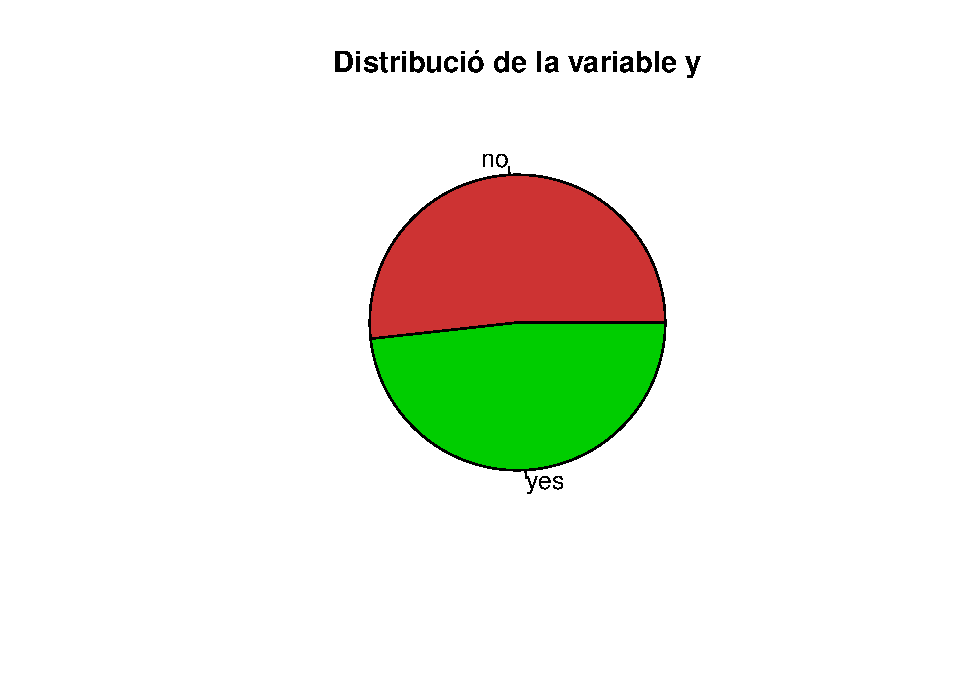
\includegraphics{Entrega2_files/figure-latex/unnamed-chunk-30-1.pdf}

\begin{Shaded}
\begin{Highlighting}[]
\FunctionTok{plot}\NormalTok{(res.hcpc\_mca, }\AttributeTok{choice =} \StringTok{"bar"}\NormalTok{)}
\end{Highlighting}
\end{Shaded}

\includegraphics{Entrega2_files/figure-latex/unnamed-chunk-30-2.pdf}

A continuació imprimirem en un factor map tots els individus agrupats
amb els diferents clusters que tenim. Podem veure com el cluster 1, 3 i
4 estan completament difgerenciats, però el cluster 2 està dispers amb
el primer i tercer. També observem com els clusters 3 i 4 tenen punts
molt desviats que provoquen que abarquin molta superfície sense
individus.

\begin{Shaded}
\begin{Highlighting}[]
\FunctionTok{fviz\_cluster}\NormalTok{(res.hcpc\_mca, }\AttributeTok{geom =} \StringTok{"point"}\NormalTok{)}
\end{Highlighting}
\end{Shaded}

\includegraphics{Entrega2_files/figure-latex/unnamed-chunk-31-1.pdf}

A continuació durem a terme la descripció de clusters envers les
variables i categories més rellevants en ells.

Primer de tot veiem les variables més relacionades amb tots els
clusters:

\begin{Shaded}
\begin{Highlighting}[]
\NormalTok{res.hcpc\_mca}\SpecialCharTok{$}\NormalTok{desc.var}\SpecialCharTok{$}\NormalTok{test.chi2}
\end{Highlighting}
\end{Shaded}

\begin{verbatim}
##                   p.value df
## job          0.000000e+00 18
## education    0.000000e+00 12
## previous     0.000000e+00  3
## poutcome     0.000000e+00  6
## month       2.749774e-235 24
## contact     9.965243e-211  3
## y           4.828120e-166  3
## marital      2.045561e-64  6
## age          6.296158e-21  9
## day_of_week  5.642845e-12 12
## housing      6.548853e-12  3
\end{verbatim}

Les següents variables són les que ens aporten més informació per
representar els clusters. Són totes variables discretes ja que es tracta
d'un anàlisis MCA:

\begin{itemize}
\tightlist
\item
  job
\item
  education
\item
  poutcome
\item
  month
\end{itemize}

Seguidament podem veure, per cadascun dels 4 clusters escollits, les
categories que els conformen. Aquests valors els relacionarem amb les
variables que hem vist que estan més relacionades per veure'n les seves
categories exactes:

\begin{Shaded}
\begin{Highlighting}[]
\NormalTok{res.hcpc\_mca}\SpecialCharTok{$}\NormalTok{desc.var}\SpecialCharTok{$}\NormalTok{category}
\end{Highlighting}
\end{Shaded}

\begin{verbatim}
## $`1`
##                                 Cla/Mod      Mod/Cla     Global       p.value
## education=basic               86.133487  66.56291685 35.1821862  0.000000e+00
## job=blue-collar               90.532081  51.44508671 25.8704453  0.000000e+00
## contact=telephone             60.247462  84.43752779 63.8056680 9.477077e-177
## month=may                     57.993351  85.32681192 66.9838057 3.520823e-146
## y=y_no                        62.098335  71.32058693 52.2874494 1.785644e-135
## marital=married               53.888000  74.87772343 63.2591093  4.968708e-55
## job=services                  76.571429  17.87461094 10.6275304  6.875358e-53
## poutcome=nonexistent          47.500536  98.44375278 94.3522267  7.002413e-34
## education=high.school         59.367194  31.70297910 24.3117409  1.989472e-28
## previous=No                   46.342469 100.00000000 98.2388664  5.871416e-24
## housing=housing_no            50.695012  55.13561583 49.5141700  4.920995e-13
## age=Adult                     50.221239  30.28012450 27.4493927  4.717230e-05
## month=jun                     58.152174   4.75767008  3.7246964  4.860564e-04
## day_of_week=tue               49.832776  26.50066696 24.2105263  6.050054e-04
## loan=loan_no                  46.290170  87.10538017 85.6680162  8.287388e-03
## month=oct                     29.268293   0.53357048  0.8299595  3.542951e-02
## day_of_week=wed               42.227378  16.18497110 17.4493927  3.217246e-02
## loan=loan_yes                 40.960452  12.89461983 14.3319838  8.287388e-03
## marital=divorced              39.196941   9.11516229 10.5870445  2.047602e-03
## age=Jove                      32.738095   2.44553135  3.4008097  6.343174e-04
## day_of_week=thu               40.081384  17.51889729 19.8987854  1.232443e-04
## month=jul                     33.587786   5.86927523  7.9554656  5.715705e-07
## age=Gran                       3.333333   0.04446421  0.6072874  3.092767e-07
## job=self-employed             29.106628   4.49088484  7.0242915  9.457441e-11
## housing=housing_yes           40.457097  44.86438417 50.4858300  4.920995e-13
## poutcome=failure              17.857143   1.55624722  3.9676113  1.144982e-16
## poutcome=success               0.000000   0.00000000  1.6801619  7.070463e-23
## previous=Yes                   0.000000   0.00000000  1.7611336  5.871416e-24
## month=mar                      2.542373   0.13339262  2.3886640  4.227342e-27
## month=nov                      8.556150   0.71142730  3.7854251  2.406330e-29
## month=aug                     11.567164   1.37839040  5.4251012  1.103349e-34
## job=management                15.466667   2.57892397  7.5910931  1.622807e-37
## marital=single                27.863777  16.00711427 26.1538462  2.705281e-51
## job=admin.                    23.123382  11.91640729 23.4615385  5.726114e-72
## month=apr                      6.378132   1.24499778  8.8866397  3.025751e-80
## y=y_yes                       27.365295  28.67941307 47.7125506 1.785644e-135
## education=professional.course  1.437700   0.40017786 12.6720648 2.460003e-162
## contact=cellular              19.574944  15.56247221 36.1943320 9.477077e-177
## job=technician                 2.002670   0.66696309 15.1619433 1.377363e-190
## education=university.degree    2.184996   1.33392619 27.7935223  0.000000e+00
##                                   v.test
## education=basic                      Inf
## job=blue-collar                      Inf
## contact=telephone              28.345623
## month=may                      25.746578
## y=y_no                         24.772245
## marital=married                15.624362
## job=services                   15.306910
## poutcome=nonexistent           12.133687
## education=high.school          11.058706
## previous=No                    10.094021
## housing=housing_no              7.227463
## age=Adult                       4.069213
## month=jun                       3.488325
## day_of_week=tue                 3.429360
## loan=loan_no                    2.640131
## month=oct                      -2.103415
## day_of_week=wed                -2.142261
## loan=loan_yes                  -2.640131
## marital=divorced               -3.083240
## age=Jove                       -3.416500
## day_of_week=thu                -3.839581
## month=jul                      -5.000584
## age=Gran                       -5.117704
## job=self-employed              -6.475379
## housing=housing_yes            -7.227463
## poutcome=failure               -8.288695
## poutcome=success               -9.846880
## previous=Yes                  -10.094021
## month=mar                     -10.781114
## month=nov                     -11.246622
## month=aug                     -12.284049
## job=management                -12.800795
## marital=single                -15.066123
## job=admin.                    -17.940188
## month=apr                     -18.969884
## y=y_yes                       -24.772245
## education=professional.course -27.151061
## contact=cellular              -28.345623
## job=technician                -29.446951
## education=university.degree         -Inf
## 
## $`2`
##                                 Cla/Mod     Mod/Cla     Global      p.value
## education=professional.course 92.971246  67.6744186 12.6720648 0.000000e+00
## job=technician                88.651535  77.2093023 15.1619433 0.000000e+00
## month=aug                     34.328358  10.6976744  5.4251012 6.104470e-12
## previous=No                   17.720997 100.0000000 98.2388664 5.046124e-08
## age=Jove-Adult                18.989959  74.7674419 68.5425101 1.140506e-05
## poutcome=nonexistent          17.850247  96.7441860 94.3522267 4.129123e-04
## day_of_week=tue               19.565217  27.2093023 24.2105263 2.520745e-02
## age=Gran                       3.333333   0.1162791  0.6072874 2.645836e-02
## age=Adult                     15.339233  24.1860465 27.4493927 1.741316e-02
## job=self-employed              9.221902   3.7209302  7.0242915 8.581173e-06
## age=Jove                       4.761905   0.9302326  3.4008097 6.527235e-07
## month=apr                      8.883827   4.5348837  8.8866397 1.253005e-07
## poutcome=success               0.000000   0.0000000  1.6801619 1.100549e-07
## previous=Yes                   0.000000   0.0000000  1.7611336 5.046124e-08
## job=unemployed                 7.495069   4.4186047 10.2631579 1.343328e-11
## job=services                   5.714286   3.4883721 10.6275304 7.876437e-17
## job=management                 3.466667   1.5116279  7.5910931 7.748804e-18
## education=university.degree    9.541151  15.2325581 27.7935223 2.408001e-21
## education=high.school          6.827644   9.5348837 24.3117409 2.928148e-33
## job=blue-collar                4.147105   6.1627907 25.8704453 3.846798e-59
## job=admin.                     2.588438   3.4883721 23.4615385 6.370328e-69
## education=basic                3.739931   7.5581395 35.1821862 6.391386e-94
##                                   v.test
## education=professional.course        Inf
## job=technician                       Inf
## month=aug                       6.877190
## previous=No                     5.449678
## age=Jove-Adult                  4.388661
## poutcome=nonexistent            3.531691
## day_of_week=tue                 2.238209
## age=Gran                       -2.219417
## age=Adult                      -2.377866
## job=self-employed              -4.450147
## age=Jove                       -4.974927
## month=apr                      -5.285590
## poutcome=success               -5.309287
## previous=Yes                   -5.449678
## job=unemployed                 -6.763892
## job=services                   -8.333082
## job=management                 -8.603253
## education=university.degree    -9.485683
## education=high.school         -12.015997
## job=blue-collar               -16.216639
## job=admin.                    -17.546104
## education=basic               -20.559018
## 
## $`3`
##                                 Cla/Mod     Mod/Cla     Global       p.value
## education=university.degree   86.598689 68.13753582 27.7935223  0.000000e+00
## job=admin.                    72.131148 47.90830946 23.4615385 7.295011e-192
## contact=cellular              58.836689 60.28653295 36.1943320 2.586108e-148
## y=y_yes                       51.803140 69.97134670 47.7125506 9.515429e-121
## month=apr                     76.765376 19.31232092  8.8866397  2.709105e-77
## job=management                79.733333 17.13467049  7.5910931  3.553602e-75
## marital=single                52.089783 38.56733524 26.1538462  2.184403e-47
## month=nov                     76.470588  8.19484241  3.7854251  1.407523e-31
## job=self-employed             60.518732 12.03438395  7.0242915  4.199892e-23
## poutcome=failure              66.326531  7.44985673  3.9676113  2.600404e-19
## month=mar                     73.728814  4.98567335  2.3886640  1.020654e-17
## previous=No                   35.936534 99.94269341 98.2388664  1.144210e-15
## age=Jove                      61.309524  5.90257880  3.4008097  3.635738e-12
## age=Gran                      93.333333  1.60458453  0.6072874  3.811565e-11
## month=aug                     54.104478  8.30945559  5.4251012  1.159896e-10
## month=jul                     50.127226 11.28939828  7.9554656  3.779458e-10
## housing=housing_yes           39.414595 56.33237822 50.4858300  1.221197e-09
## day_of_week=thu               40.488301 22.80802292 19.8987854  1.721074e-04
## marital=divorced              42.447419 12.72206304 10.5870445  3.672714e-04
## job=unemployed                42.406312 12.32091691 10.2631579  4.992983e-04
## day_of_week=wed               39.443155 19.48424069 17.4493927  5.647987e-03
## month=oct                     51.219512  1.20343840  0.8299595  3.806523e-02
## age=Adult                     32.669617 25.38681948 27.4493927  1.608590e-02
## month=jun                     25.543478  2.69340974  3.7246964  3.955253e-03
## education=high.school         31.806828 21.89111748 24.3117409  3.241826e-03
## poutcome=nonexistent          34.649217 92.55014327 94.3522267  6.875285e-05
## day_of_week=tue               29.933110 20.51575931 24.2105263  6.301578e-06
## housing=housing_no            31.152903 43.66762178 49.5141700  1.221197e-09
## previous=Yes                   1.149425  0.05730659  1.7611336  1.144210e-15
## poutcome=success               0.000000  0.00000000  1.6801619  1.336576e-16
## job=services                  16.190476  4.87106017 10.6275304  1.268130e-24
## marital=married               27.200000 48.71060172 63.2591093  1.050906e-54
## job=technician                 6.542056  2.80802292 15.1619433  3.344219e-88
## education=professional.course  3.194888  1.14613181 12.6720648  9.838051e-96
## y=y_no                        20.286489 30.02865330 52.2874494 9.515429e-121
## month=may                     23.209429 44.01146132 66.9838057 8.495490e-140
## contact=telephone             21.986041 39.71346705 63.8056680 2.586108e-148
## job=blue-collar                3.990610  2.92263610 25.8704453 3.266085e-204
## education=basic                8.745685  8.71060172 35.1821862 1.448069e-207
##                                   v.test
## education=university.degree          Inf
## job=admin.                     29.546446
## contact=cellular               25.936442
## y=y_yes                        23.365829
## month=apr                      18.609144
## job=management                 18.345995
## marital=single                 14.459480
## month=nov                      11.691575
## job=self-employed               9.899112
## poutcome=failure                8.984446
## month=mar                       8.571591
## previous=No                     8.010309
## age=Jove                        6.950663
## age=Gran                        6.611223
## month=aug                       6.444490
## month=jul                       6.262874
## housing=housing_yes             6.077436
## day_of_week=thu                 3.756789
## marital=divorced                3.562549
## job=unemployed                  3.481133
## day_of_week=wed                 2.767547
## month=oct                       2.074152
## age=Adult                      -2.406961
## month=jun                      -2.881709
## education=high.school          -2.943826
## poutcome=nonexistent           -3.980561
## day_of_week=tue                -4.516010
## housing=housing_no             -6.077436
## previous=Yes                   -8.010309
## poutcome=success               -8.270269
## job=services                  -10.243317
## marital=married               -15.576540
## job=technician                -19.909834
## education=professional.course -20.760576
## y=y_no                        -23.365829
## month=may                     -25.170195
## contact=telephone             -25.936442
## job=blue-collar               -30.492603
## education=basic               -30.744506
## 
## $`4`
##                          Cla/Mod    Mod/Cla    Global       p.value     v.test
## previous=Yes          98.8505747 100.000000  1.761134 9.693892e-186  29.065884
## poutcome=success     100.0000000  96.511628  1.680162 2.126492e-177  28.398230
## contact=cellular       4.4742729  93.023256 36.194332  5.878562e-29  11.167541
## y=y_yes                3.6487060 100.000000 47.712551  1.008897e-28  11.119452
## month=apr              7.9726651  40.697674  8.886640  1.072676e-15   8.018244
## day_of_week=thu        3.7639878  43.023256 19.898785  9.257787e-07   4.906793
## job=technician         2.8037383  24.418605 15.161943  2.337339e-02   2.267276
## month=jun              0.0000000   0.000000  3.724696  3.712800e-02  -2.084354
## month=may              1.3901481  53.488372 66.983806  9.052054e-03  -2.610082
## month=aug              0.0000000   0.000000  5.425101  7.908101e-03  -2.655968
## month=jul              0.0000000   0.000000  7.955466  7.511337e-04  -3.370201
## day_of_week=tue        0.6688963   9.302326 24.210526  4.297599e-04  -3.521100
## y=y_no                 0.0000000   0.000000 52.287449  1.008897e-28 -11.119452
## contact=telephone      0.1903553   6.976744 63.805668  5.878562e-29 -11.167541
## poutcome=nonexistent   0.0000000   0.000000 94.352227 4.020961e-114 -22.704752
## previous=No            0.0000000   0.000000 98.238866 9.693892e-186 -29.065884
\end{verbatim}

\begin{itemize}
\item
  Cluster 1

  \begin{itemize}
  \item
    job

    \begin{enumerate}
    \def\labelenumi{\arabic{enumi}.}
    \item
      blue.collar (51,45\%)
    \item
      services (17,87\%)
    \item
      admin (11.92\%) (de forma negativa)
    \end{enumerate}
  \item
    education

    \begin{enumerate}
    \def\labelenumi{\arabic{enumi}.}
    \item
      basic (66,56\%)
    \item
      high.school (31,7\%)
    \end{enumerate}
  \item
    month

    \begin{enumerate}
    \def\labelenumi{\arabic{enumi}.}
    \tightlist
    \item
      may (85,33\%)
    \end{enumerate}
  \end{itemize}
\end{itemize}

Com a informació addicional, comentar que cap dels individus dins del
cluster ha estat contactat previament (previous=no), això provoca que hi
hagi un 0\% de poutcome=success.

\begin{itemize}
\item
  Cluster 2

  \begin{itemize}
  \item
    job

    \begin{enumerate}
    \def\labelenumi{\arabic{enumi}.}
    \tightlist
    \item
      technician (77.21\%)
    \end{enumerate}
  \item
    education

    \begin{enumerate}
    \def\labelenumi{\arabic{enumi}.}
    \item
      professional.course (67.67\%): Veiem una clara relació entre
      aquests nivells d'estudis i la categoria technician de la variable
      job: la majoria de fp estan destinades a feines tècniques.
    \item
      university.degree (15.23\%) (de forma negativa)
    \end{enumerate}
  \item
    month

    \begin{enumerate}
    \def\labelenumi{\arabic{enumi}.}
    \item
      aug (10,69\%)
    \item
      apr (4,53\%) (de forma negativa)
    \end{enumerate}

    En aquest cluster la variable té molt poc pes.
  \end{itemize}
\item
  Cluster 3

  \begin{itemize}
  \item
    job

    \begin{enumerate}
    \def\labelenumi{\arabic{enumi}.}
    \item
      admin (47,91\%)
    \item
      management (17,13\%)
    \item
      self-employed (12,03\%)
    \end{enumerate}

    Aquestes tres categories estan bastant relacionades amb el tipus de
    feina que són, ja que feines administratives, de control i d'autònom
    són similars.
  \item
    education

    \begin{enumerate}
    \def\labelenumi{\arabic{enumi}.}
    \item
      university.degree (68.14\%): Aquesta categoria esta bastant
      relacionada amb els nivells de job descrits anteriorment, ja que
      són posicions de feina altes i aquí es descriu el nivell més alt
      d'estudis registrat.
    \item
      high.school (21.89\%) (de forma negativa)
    \end{enumerate}
  \item
    month

    \begin{enumerate}
    \def\labelenumi{\arabic{enumi}.}
    \item
      may (44,01\%) (de forma negativa)
    \item
      apr (19,31\%)
    \item
      jul (11,29\%)
    \item
      aug (8,31\%)
    \end{enumerate}
  \end{itemize}
\item
  Cluster 4

  \begin{itemize}
  \item
    month

    \begin{enumerate}
    \def\labelenumi{\arabic{enumi}.}
    \item
      may (53,49\%) (de forma negativa)
    \item
      apr (40,70\%)
    \end{enumerate}
  \end{itemize}
\end{itemize}

En aquest últim cluster, com que tenen un gran pes previous i poutcome,
les variables job i education no són representatives. En el cas de
previous, la categoria més significant és yes (100\%) i de poutcome és
success (96,51\%). Destacar també que tots els poutcome=success es
troben en aquest cluster.

\begin{itemize}
\tightlist
\item
  Cut quality
\end{itemize}

La qualitat de la partició amb 4 clusters és del 48.2918107\%.

\hypertarget{parangons-and-class-specific-individuals}{%
\subsubsection{Parangons and class-specific
individuals}\label{parangons-and-class-specific-individuals}}

En aquest apartat podem observar els individus més cercans i més
allunyats dels centroides de cada cluster.

A la taula següent podem veure, per cada cluster, els 5 individus més
cercans als centroides amb les respectives distàncies:

\begin{Shaded}
\begin{Highlighting}[]
\NormalTok{res.hcpc\_mca}\SpecialCharTok{$}\NormalTok{desc.ind}\SpecialCharTok{$}\NormalTok{para}
\end{Highlighting}
\end{Shaded}

\begin{verbatim}
## Cluster: 1
##        218       2140        162         70        217 
## 0.07651285 0.07651285 0.07651285 0.07651285 0.08021202 
## ------------------------------------------------------------ 
## Cluster: 2
##     21748     19754      2385      2006     35970 
## 0.2762256 0.2964458 0.2977149 0.3060090 0.3098983 
## ------------------------------------------------------------ 
## Cluster: 3
##     12566     17809     25995     14696     15936 
## 0.1232529 0.1243103 0.1244148 0.1356608 0.1464823 
## ------------------------------------------------------------ 
## Cluster: 4
##     25854     30502     33387     30464     34649 
## 0.3519480 0.3537620 0.3607975 0.4241063 0.4299914
\end{verbatim}

A la taula següent podem veure, per cada cluster, els 5 individus més
distants als centroides amb les respectives distàncies:

\begin{Shaded}
\begin{Highlighting}[]
\NormalTok{res.hcpc\_mca}\SpecialCharTok{$}\NormalTok{desc.ind}\SpecialCharTok{$}\NormalTok{dist}
\end{Highlighting}
\end{Shaded}

\begin{verbatim}
## Cluster: 1
##    30005     1760     1730     1764     1725 
## 1.941382 1.577068 1.570114 1.522564 1.522564 
## ------------------------------------------------------------ 
## Cluster: 2
##    27724    30302    27767    30141    19249 
## 1.999976 1.534193 1.516153 1.510455 1.502705 
## ------------------------------------------------------------ 
## Cluster: 3
##    28615    28541    29982    30001    30384 
## 2.643395 2.627127 2.507550 2.507550 2.368233 
## ------------------------------------------------------------ 
## Cluster: 4
##    30154    28677    30236    30239    30208 
## 3.528231 3.510440 3.508366 3.506306 3.506113
\end{verbatim}

\begin{Shaded}
\begin{Highlighting}[]
\NormalTok{res.hcpc\_mca}\SpecialCharTok{$}\NormalTok{data.clust[}\FunctionTok{which}\NormalTok{(}\FunctionTok{rownames}\NormalTok{(res.hcpc\_mca}\SpecialCharTok{$}\NormalTok{data.clust)}\SpecialCharTok{\%in\%}\NormalTok{names}
\NormalTok{                              (res.hcpc\_mca}\SpecialCharTok{$}\NormalTok{desc.ind}\SpecialCharTok{$}\NormalTok{para[[}\DecValTok{1}\NormalTok{]])),]}
\end{Highlighting}
\end{Shaded}

\begin{verbatim}
##         y        age         job marital education     housing     loan
## 217  y_no Jove-Adult blue-collar  single     basic housing_yes  loan_no
## 218  y_no Jove-Adult blue-collar  single     basic housing_yes loan_yes
## 2140 y_no Jove-Adult blue-collar  single     basic housing_yes loan_yes
## 162  y_no Jove-Adult blue-collar  single     basic housing_yes loan_yes
## 70   y_no Jove-Adult blue-collar  single     basic housing_yes loan_yes
##        contact month day_of_week previous    poutcome clust
## 217  telephone   may         mon       No nonexistent     1
## 218  telephone   may         mon       No nonexistent     1
## 2140 telephone   may         mon       No nonexistent     1
## 162  telephone   may         mon       No nonexistent     1
## 70   telephone   may         mon       No nonexistent     1
\end{verbatim}

\begin{Shaded}
\begin{Highlighting}[]
\NormalTok{res.hcpc\_mca}\SpecialCharTok{$}\NormalTok{data.clust[}\FunctionTok{which}\NormalTok{(}\FunctionTok{rownames}\NormalTok{(res.hcpc\_mca}\SpecialCharTok{$}\NormalTok{data.clust)}\SpecialCharTok{\%in\%}\NormalTok{names}
\NormalTok{                              (res.hcpc\_mca}\SpecialCharTok{$}\NormalTok{desc.ind}\SpecialCharTok{$}\NormalTok{dist[[}\DecValTok{1}\NormalTok{]])),]}
\end{Highlighting}
\end{Shaded}

\begin{verbatim}
##           y  age        job marital   education     housing     loan   contact
## 30005 y_yes Gran unemployed married       basic housing_yes  loan_no telephone
## 1764  y_yes Jove   services  single high.school housing_yes  loan_no telephone
## 1725   y_no Jove   services  single high.school housing_yes  loan_no telephone
## 1730   y_no Jove   services  single high.school  housing_no  loan_no telephone
## 1760   y_no Jove   services  single high.school  housing_no loan_yes telephone
##       month day_of_week previous    poutcome clust
## 30005   apr         tue       No nonexistent     1
## 1764    may         fri       No nonexistent     1
## 1725    may         fri       No nonexistent     1
## 1730    may         fri       No nonexistent     1
## 1760    may         fri       No nonexistent     1
\end{verbatim}

\begin{Shaded}
\begin{Highlighting}[]
\NormalTok{res.hcpc\_mca}\SpecialCharTok{$}\NormalTok{data.clust[}\FunctionTok{which}\NormalTok{(}\FunctionTok{rownames}\NormalTok{(res.hcpc\_mca}\SpecialCharTok{$}\NormalTok{data.clust)}\SpecialCharTok{\%in\%}\NormalTok{names}
\NormalTok{                              (res.hcpc\_mca}\SpecialCharTok{$}\NormalTok{desc.ind}\SpecialCharTok{$}\NormalTok{para[[}\DecValTok{2}\NormalTok{]])),]}
\end{Highlighting}
\end{Shaded}

\begin{verbatim}
##           y        age           job marital           education     housing
## 19754 y_yes Jove-Adult    technician married         high.school  housing_no
## 21748 y_yes Jove-Adult      services married professional.course  housing_no
## 35970 y_yes Jove-Adult    technician married professional.course  housing_no
## 2006   y_no      Adult    technician  single professional.course housing_yes
## 2385   y_no Jove-Adult self-employed  single professional.course housing_yes
##           loan   contact month day_of_week previous    poutcome clust
## 19754  loan_no telephone   aug         fri       No nonexistent     2
## 21748  loan_no  cellular   aug         tue       No nonexistent     2
## 35970  loan_no  cellular   may         mon       No nonexistent     2
## 2006   loan_no telephone   may         mon       No nonexistent     2
## 2385  loan_yes telephone   may         tue       No nonexistent     2
\end{verbatim}

\begin{Shaded}
\begin{Highlighting}[]
\NormalTok{res.hcpc\_mca}\SpecialCharTok{$}\NormalTok{data.clust[}\FunctionTok{which}\NormalTok{(}\FunctionTok{rownames}\NormalTok{(res.hcpc\_mca}\SpecialCharTok{$}\NormalTok{data.clust)}\SpecialCharTok{\%in\%}\NormalTok{names}
\NormalTok{                              (res.hcpc\_mca}\SpecialCharTok{$}\NormalTok{desc.ind}\SpecialCharTok{$}\NormalTok{dist[[}\DecValTok{2}\NormalTok{]])),]}
\end{Highlighting}
\end{Shaded}

\begin{verbatim}
##           y        age        job marital           education     housing
## 27767 y_yes Jove-Adult technician  single professional.course housing_yes
## 19249 y_yes Jove-Adult technician  single professional.course housing_yes
## 30141 y_yes Jove-Adult technician married professional.course housing_yes
## 30302 y_yes      Adult technician married professional.course housing_yes
## 27724 y_yes       Gran technician married professional.course housing_yes
##           loan  contact month day_of_week previous    poutcome clust
## 27767 loan_yes cellular   mar         fri       No nonexistent     2
## 19249 loan_yes cellular   aug         wed       No nonexistent     2
## 30141  loan_no cellular   apr         thu       No     failure     2
## 30302 loan_yes cellular   apr         thu       No     failure     2
## 27724  loan_no cellular   mar         tue       No nonexistent     2
\end{verbatim}

\begin{Shaded}
\begin{Highlighting}[]
\NormalTok{res.hcpc\_mca}\SpecialCharTok{$}\NormalTok{data.clust[}\FunctionTok{which}\NormalTok{(}\FunctionTok{rownames}\NormalTok{(res.hcpc\_mca}\SpecialCharTok{$}\NormalTok{data.clust)}\SpecialCharTok{\%in\%}\NormalTok{names}
\NormalTok{                              (res.hcpc\_mca}\SpecialCharTok{$}\NormalTok{desc.ind}\SpecialCharTok{$}\NormalTok{para[[}\DecValTok{3}\NormalTok{]])),]}
\end{Highlighting}
\end{Shaded}

\begin{verbatim}
##           y        age        job marital         education     housing    loan
## 17809 y_yes Jove-Adult     admin. married university.degree  housing_no loan_no
## 15936 y_yes Jove-Adult     admin. married university.degree  housing_no loan_no
## 12566 y_yes Jove-Adult management married       high.school housing_yes loan_no
## 25995 y_yes      Adult     admin. married       high.school  housing_no loan_no
## 14696 y_yes Jove-Adult management married       high.school housing_yes loan_no
##        contact month day_of_week previous    poutcome clust
## 17809 cellular   jul         tue       No nonexistent     3
## 15936 cellular   jul         mon       No nonexistent     3
## 12566 cellular   jul         mon       No nonexistent     3
## 25995 cellular   nov         wed       No nonexistent     3
## 14696 cellular   jul         tue       No nonexistent     3
\end{verbatim}

\begin{Shaded}
\begin{Highlighting}[]
\NormalTok{res.hcpc\_mca}\SpecialCharTok{$}\NormalTok{data.clust[}\FunctionTok{which}\NormalTok{(}\FunctionTok{rownames}\NormalTok{(res.hcpc\_mca}\SpecialCharTok{$}\NormalTok{data.clust)}\SpecialCharTok{\%in\%}\NormalTok{names}
\NormalTok{                              (res.hcpc\_mca}\SpecialCharTok{$}\NormalTok{desc.ind}\SpecialCharTok{$}\NormalTok{dist[[}\DecValTok{3}\NormalTok{]])),]}
\end{Highlighting}
\end{Shaded}

\begin{verbatim}
##           y  age        job marital education     housing     loan  contact
## 30384 y_yes Gran unemployed  single     basic housing_yes  loan_no cellular
## 28541 y_yes Gran unemployed married     basic  housing_no  loan_no cellular
## 29982 y_yes Gran unemployed married     basic  housing_no  loan_no cellular
## 30001 y_yes Gran unemployed married     basic  housing_no  loan_no cellular
## 28615 y_yes Gran unemployed married     basic  housing_no loan_yes cellular
##       month day_of_week previous    poutcome clust
## 30384   apr         thu       No nonexistent     3
## 28541   apr         wed       No     failure     3
## 29982   apr         tue       No     failure     3
## 30001   apr         tue       No     failure     3
## 28615   apr         wed       No     failure     3
\end{verbatim}

\begin{Shaded}
\begin{Highlighting}[]
\NormalTok{res.hcpc\_mca}\SpecialCharTok{$}\NormalTok{data.clust[}\FunctionTok{which}\NormalTok{(}\FunctionTok{rownames}\NormalTok{(res.hcpc\_mca}\SpecialCharTok{$}\NormalTok{data.clust)}\SpecialCharTok{\%in\%}\NormalTok{names}
\NormalTok{                              (res.hcpc\_mca}\SpecialCharTok{$}\NormalTok{desc.ind}\SpecialCharTok{$}\NormalTok{para[[}\DecValTok{4}\NormalTok{]])),]}
\end{Highlighting}
\end{Shaded}

\begin{verbatim}
##           y        age         job marital   education     housing     loan
## 34649 y_yes Jove-Adult  technician  single       basic housing_yes  loan_no
## 25854 y_yes Jove-Adult blue-collar  single high.school housing_yes  loan_no
## 30464 y_yes Jove-Adult  unemployed married high.school  housing_no  loan_no
## 30502 y_yes Jove-Adult  unemployed married high.school housing_yes  loan_no
## 33387 y_yes Jove-Adult      admin.  single       basic  housing_no loan_yes
##        contact month day_of_week previous poutcome clust
## 34649 cellular   may         thu      Yes  success     4
## 25854 cellular   nov         wed      Yes  success     4
## 30464 cellular   may         mon      Yes  success     4
## 30502 cellular   may         mon      Yes  success     4
## 33387 cellular   may         tue      Yes  success     4
\end{verbatim}

\begin{Shaded}
\begin{Highlighting}[]
\NormalTok{res.hcpc\_mca}\SpecialCharTok{$}\NormalTok{data.clust[}\FunctionTok{which}\NormalTok{(}\FunctionTok{rownames}\NormalTok{(res.hcpc\_mca}\SpecialCharTok{$}\NormalTok{data.clust)}\SpecialCharTok{\%in\%}\NormalTok{names}
\NormalTok{                              (res.hcpc\_mca}\SpecialCharTok{$}\NormalTok{desc.ind}\SpecialCharTok{$}\NormalTok{dist[[}\DecValTok{4}\NormalTok{]])),]}
\end{Highlighting}
\end{Shaded}

\begin{verbatim}
##           y        age         job marital           education     housing
## 30239 y_yes      Adult  technician married professional.course housing_yes
## 28677 y_yes Jove-Adult blue-collar married               basic  housing_no
## 30208 y_yes Jove-Adult  technician  single professional.course housing_yes
## 30154 y_yes Jove-Adult    services married         high.school housing_yes
## 30236 y_yes      Adult  technician married professional.course housing_yes
##           loan  contact month day_of_week previous poutcome clust
## 30239  loan_no cellular   apr         thu      Yes  success     4
## 28677  loan_no cellular   apr         thu      Yes  success     4
## 30208  loan_no cellular   apr         thu      Yes  success     4
## 30154  loan_no cellular   apr         thu      Yes  success     4
## 30236 loan_yes cellular   apr         thu      Yes  success     4
\end{verbatim}

En les taules anteriors hem pogut veure els valors de les variables que
tenen els individus més propers i llunyans de cada cluster. D'aquí podem
treure les següents conclusions:

\begin{itemize}
\item
  Els individus més propers, tenen valors de les variables corresponents
  amb les categories vistes a la descripció de clusters, per tant, té
  sentit que siguin els individus més cercans al centroide.
\item
  Els individus més llunyans, tenen valors de les variables contraris
  amb les categories vistes a la descripció de clusters, per tant, té
  sentit que siguin els individus més distants al centroide.
\end{itemize}

\end{document}
